% =============================================================
%  FPGA与VHDL考试变式题解析册
%  每题含：分析→状态图→设计→VHDL→Testbench→波形→秒杀
% =============================================================

\documentclass[12pt,a4paper,openany]{ctexbook}

\usepackage{fontspec}
\setmainfont{Times New Roman}
\setCJKmainfont{SimSun}[AutoFakeBold=2.5]
\setCJKsansfont{SimHei}

\usepackage[top=2.5cm,bottom=2.5cm,left=2.5cm,right=2.5cm]{geometry}
\usepackage{amsmath,amssymb}
\usepackage{tikz}
\usepackage{circuitikz}
\usetikzlibrary{arrows,shapes,positioning,calc,automata,patterns}

\usepackage{tabularx,booktabs,multirow,makecell,colortbl}
\usepackage{listings,xcolor,enumitem,caption,float}

% VHDL listings config
\definecolor{vhdlcomment}{rgb}{0.0,0.5,0.0}
\definecolor{vhdlkeyword}{rgb}{0.0,0.0,0.8}
\definecolor{vhdlstring}{rgb}{0.6,0.1,0.1}
\definecolor{vhdlnumber}{rgb}{0.5,0.5,0.5}
\definecolor{vhdlbackground}{rgb}{0.97,0.97,0.97}


\lstset{language={},
  basicstyle=\ttfamily\footnotesize,
  numbers=left,numberstyle=\tiny\color{vhdlnumber},
  backgroundcolor=\color{vhdlbackground},frame=single,tabsize=2,
  breaklines=true,showstringspaces=false}

\usepackage[colorlinks=true,linkcolor=blue!60!black,urlcolor=blue!60!black]{hyperref}

% Custom environments (use simple framed boxes to avoid lstlisting/NewEnviron conflicts)
\usepackage{framed,color}

\newenvironment{solution}[1][完整解答]
  {\begin{oframed}\textbf{\large #1}\\[3pt]}
  {\end{oframed}}

\newenvironment{quickkill}[1][秒杀口诀]
  {\begin{oframed}\textbf{\textcolor{red!70!black}{#1}}\\[3pt]}
  {\end{oframed}}

\title{\Huge\textbf{FPGA与VHDL考试\\变式题解析册}}
\author{}
\date{\today}

\begin{document}
\maketitle
\tableofcontents

% =============================================================
\part{计数器变式题解析（20题）}
\chapter{计数器变式题（20题完整解析）}

% ============================================================
\section{题1：模7计数器}

\textbf{题目}：设计模7计数器（0→1→...→6→0→...），写VHDL和Testbench。

\begin{solution}[完整解答]

\textbf{【分析】}
$N=7$，位宽 $k=\lceil\log_2 7\rceil=3$。清零条件：$cnt = 6(110)$。

\textbf{【状态图】}
\begin{center}
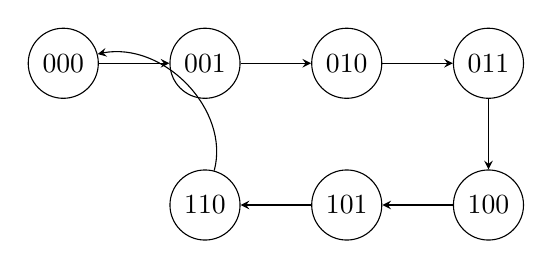
\begin{tikzpicture}[->,>=stealth,node distance=1.8cm]
\node[draw,circle] (s0) {000}; \node[draw,circle,right of=s0] (s1) {001};
\node[draw,circle,right of=s1] (s2) {010}; \node[draw,circle,right of=s2] (s3) {011};
\node[draw,circle,below of=s3] (s4) {100}; \node[draw,circle,left of=s4] (s5) {101};
\node[draw,circle,left of=s5] (s6) {110};
\draw (s0)--(s1); \draw (s1)--(s2); \draw (s2)--(s3);
\draw (s3)--(s4); \draw (s4)--(s5); \draw (s5)--(s6);
\draw (s6) edge[bend right=60] (s0);
\end{tikzpicture}
\end{center}

\textbf{【状态转移表】}
\begin{center}
\begin{tabular}{|c|c|c|}
\hline 当前状态(十进制) & 当前状态(二进制) & 下一状态 \\
\hline 0 & 000 & 001 \\ \hline 1 & 001 & 010 \\
\hline 2 & 010 & 011 \\ \hline 3 & 011 & 100 \\
\hline 4 & 100 & 101 \\ \hline 5 & 101 & 110 \\
\hline 6 & 110 & \textbf{000}（清零）\\
\hline
\end{tabular}
\end{center}

\textbf{【VHDL】}
\begin{lstlisting}
library ieee;
use ieee.std_logic_1164.all;
use ieee.std_logic_unsigned.all;

entity counter_mod7 is
  port (clk, rst_n : in std_logic;
        count : out std_logic_vector(2 downto 0);
        carry : out std_logic);
end counter_mod7;

architecture behavioral of counter_mod7 is
  signal cnt : std_logic_vector(2 downto 0);
begin
  process(clk, rst_n)
  begin
    if rst_n = '0' then
      cnt <= "000";
    elsif rising_edge(clk) then
      if cnt = "110" then     -- =6
        cnt <= "000";
      else
        cnt <= cnt + 1;
      end if;
    end if;
  end process;
  count <= cnt;
  carry <= '1' when cnt = "110" else '0';
end behavioral;
\end{lstlisting}

\textbf{【Testbench】}
\begin{lstlisting}
entity counter_mod7_tb is end entity;
architecture test of counter_mod7_tb is
  signal clk, rst_n, carry : std_logic;
  signal count : std_logic_vector(2 downto 0);
  constant T : time := 20 ns;
begin
  uut: entity work.counter_mod7 port map(clk, rst_n, count, carry);
  clk <= not clk after T/2;
  process begin
    rst_n <= '0'; wait for 30 ns;
    rst_n <= '1';
    -- 观察两个完整循环(14拍)
    wait for 14*T;
    wait;
  end process;
end test;
\end{lstlisting}

\textbf{【波形分析】}
\begin{center}
\begin{tabular}{|c|c|c|}
\hline 时钟拍 & count(二进制) & 十进制 \\ \hline
1 & 001 & 1 \\ \hline
2 & 010 & 2 \\ \hline
...&...&...\\ \hline
6 & 110 & 6 \\ \hline
7 & 000 & 0（carry=1！）\\ \hline
8 & 001 & 1（新循环）\\ \hline
\end{tabular}
\end{center}
验证：第7拍count归零且carry=1，第8拍count=1，循环正确。

\end{solution}

\begin{quickkill}
$k=\lceil\log_2 N\rceil$，清零条件=$N{-}1$。套模板：\texttt{if cnt = N-1 then cnt<=0; else cnt<=cnt+1;}
\end{quickkill}


% ============================================================
\section{题2：模5计数器}

\textbf{题目}：设计模5计数器（0→1→2→3→4→0→...），写出完整VHDL。

\begin{solution}[完整解答]

\textbf{【分析】}$N=5$，$k=\lceil\log_2 5\rceil=3$位。清零条件：$cnt=4(100)$。

\textbf{【状态序列】}$000 \to 001 \to 010 \to 011 \to 100 \to 000$

\textbf{【VHDL】}
\begin{lstlisting}
library ieee;
use ieee.std_logic_1164.all;
use ieee.std_logic_unsigned.all;

entity counter_mod5 is
  port (clk, rst_n : in std_logic;
        count : out std_logic_vector(2 downto 0);
        carry : out std_logic);
end counter_mod5;

architecture behavioral of counter_mod5 is
  signal cnt : std_logic_vector(2 downto 0);
begin
  process(clk, rst_n)
  begin
    if rst_n = '0' then cnt <= "000";
    elsif rising_edge(clk) then
      if cnt = "100" then cnt <= "000";  -- =4清零
      else cnt <= cnt + 1;
      end if;
    end if;
  end process;
  count <= cnt;
  carry <= '1' when cnt = "100" else '0';
end behavioral;
\end{lstlisting}

\textbf{【验证】}5拍一个循环。第5拍cnt=100(4)且carry=1，下一拍归零。

\textbf{【注意】}状态101/110/111（5-7）永远不会出现——这是正常现象，3位能表示0-7但只用了0-4。

\end{solution}


% ============================================================
\section{题3：模12计数器}

\textbf{题目}：设计模12计数器（0→1→...→11→0），并解释为什么不能自然溢出。

\begin{solution}[完整解答]

\textbf{【分析】}$N=12$，$k=\lceil\log_2 12\rceil=4$位。清零条件：$cnt=11(1011)$。

\textbf{【为什么不能自然溢出】}4位自然溢出=模16。如果不加清零逻辑，1111+1=0000，会经过16个状态而不是12个。必须显式在cnt=11时清零。

\textbf{【VHDL】}
\begin{lstlisting}
library ieee;
use ieee.std_logic_1164.all;
use ieee.std_logic_unsigned.all;

entity counter_mod12 is
  port (clk, rst_n : in std_logic;
        count : out std_logic_vector(3 downto 0);
        carry : out std_logic);
end counter_mod12;

architecture behavioral of counter_mod12 is
  signal cnt : std_logic_vector(3 downto 0);
begin
  process(clk, rst_n)
  begin
    if rst_n = '0' then cnt <= "0000";
    elsif rising_edge(clk) then
      if cnt = "1011" then cnt <= "0000";  -- =11清零
      else cnt <= cnt + 1;
      end if;
    end if;
  end process;
  count <= cnt;
  carry <= '1' when cnt = "1011" else '0';
end behavioral;
\end{lstlisting}

\textbf{【Testbench关键验证点】}
\begin{itemize}
  \item 第12拍：cnt=1011(11)，carry=1
  \item 第13拍：cnt=0000(0)（归零！）
  \item 第14拍：cnt=0001(1)（新循环开始）
\end{itemize}

\end{solution}


% ============================================================
\section{题4：模13计数器}

\textbf{题目}：设计模13计数器（0→1→...→12→0）。

\begin{solution}[完整解答]

\textbf{【分析】}$N=13$，$k=\lceil\log_2 13\rceil=4$位。清零条件：$cnt=12(1100)$。

\textbf{【VHDL】}
\begin{lstlisting}
signal cnt : std_logic_vector(3 downto 0);
-- 清零条件：cnt = "1100"  (=12)
 if cnt = "1100" then cnt <= "0000";
else cnt <= cnt + 1; end if;
\end{lstlisting}

\textbf{【完整状态序列】}
$$0000\to0001\to0010\to0011\to0100\to0101\to0110\to0111$$
$$\to1000\to1001\to1010\to1011\to1100\to0000$$

共13个状态。状态1101/1110/1111（13-15）永不出现。

\end{solution}


% ============================================================
\section{题5：模24计数器}

\textbf{题目}：设计模24计数器（0→1→...→23→0），用于小时计数器。

\begin{solution}[完整解答]

\textbf{【分析】}$N=24$，$k=\lceil\log_2 24\rceil=5$位。清零条件：$cnt=23(10111)$。

\textbf{【VHDL】}
\begin{lstlisting}
library ieee;
use ieee.std_logic_1164.all;
use ieee.std_logic_unsigned.all;

entity counter_mod24 is
  port (clk, rst_n : in std_logic;
        count : out std_logic_vector(4 downto 0);
        carry : out std_logic);
end counter_mod24;

architecture behavioral of counter_mod24 is
  signal cnt : std_logic_vector(4 downto 0);
begin
  process(clk, rst_n)
  begin
    if rst_n = '0' then cnt <= (others => '0');
    elsif rising_edge(clk) then
      if cnt = "10111" then cnt <= (others => '0');
      else cnt <= cnt + 1;
      end if;
    end if;
  end process;
  count <= cnt;
  carry <= '1' when cnt = "10111" else '0';
end behavioral;
\end{lstlisting}

\textbf{【状态范围】}00000(0)→00001(1)→...→10111(23)→00000(0)

注意：5位最多表示31，剩余8个状态(11000-11111)永不出现。

\textbf{【应用】}数字钟的小时计数器。

\end{solution}


% ============================================================
\section{题6：模60计数器（二进制）}

\textbf{题目}：设计模60计数器（0→1→...→59→0），用于秒/分计数器。

\begin{solution}[完整解答]

\textbf{【分析】}$N=60$，$k=\lceil\log_2 60\rceil=6$位。清零条件：$cnt=59(111011)$。

\textbf{【VHDL】}
\begin{lstlisting}
library ieee;
use ieee.std_logic_1164.all;
use ieee.std_logic_unsigned.all;

entity counter_mod60 is
  port (clk, rst_n : in std_logic;
        count : out std_logic_vector(5 downto 0);
        carry : out std_logic);
end counter_mod60;

architecture behavioral of counter_mod60 is
  signal cnt : std_logic_vector(5 downto 0);
begin
  process(clk, rst_n)
  begin
    if rst_n = '0' then cnt <= (others => '0');
    elsif rising_edge(clk) then
      if cnt = "111011" then cnt <= (others => '0');
      else cnt <= cnt + 1;
      end if;
    end if;
  end process;
  count <= cnt;
  carry <= '1' when cnt = "111011" else '0';
end behavioral;
\end{lstlisting}

\textbf{【二进制 vs BCD模60】}
\begin{itemize}
  \item 二进制模60：一个6位整体计数器（如本题）
  \item BCD模60：十位(模6)+个位(模10)级联
  \item 考试中要注意区分"二进制模60"和"BCD模60"
\end{itemize}

\end{solution}


% ============================================================
\section{题7：模10 BCD计数器}

\textbf{题目}：设计模10 BCD计数器（0→1→...→9→0）。个位，4位输出，BCD编码。

\begin{solution}[完整解答]

\textbf{【分析】}$N=10$，$k=4$位。状态：0000→0001→...→1001→0000。状态1010-1111不允许出现。

\textbf{【VHDL】}
\begin{lstlisting}
library ieee;
use ieee.std_logic_1164.all;
use ieee.std_logic_unsigned.all;

entity bcd_counter_mod10 is
  port (clk, rst_n : in std_logic;
        bcd : out std_logic_vector(3 downto 0);
        carry : out std_logic);
end bcd_counter_mod10;

architecture behavioral of bcd_counter_mod10 is
  signal cnt : std_logic_vector(3 downto 0);
begin
  process(clk, rst_n)
  begin
    if rst_n = '0' then cnt <= "0000";
    elsif rising_edge(clk) then
      if cnt = "1001" then cnt <= "0000";  -- =9清零
      else cnt <= cnt + 1;
      end if;
    end if;
  end process;
  bcd <= cnt;
  carry <= '1' when cnt = "1001" else '0';
end behavioral;
\end{lstlisting}

\textbf{【关键】}与普通模10计数器的区别：BCD的每个十进制位是独立4位，显示友好。

\end{solution}


% ============================================================
\section{题8：模60 BCD计数器（级联方案）}

\textbf{题目}：设计BCD模60计数器，个位(模10)+十位(模6)。输出十位和个位各4位BCD码。

\begin{solution}[完整解答]

\textbf{【分析】}
个位：模10，满9→清零并向十位进位。
十位：收到进位+1，十位模6（0-5）。
整体清零条件：十位=5且个位=9（即59）。

\textbf{【VHDL】}
\begin{lstlisting}
library ieee;
use ieee.std_logic_1164.all;
use ieee.std_logic_unsigned.all;

entity bcd_mod60 is
  port (clk, rst_n : in std_logic;
        tens, units : out std_logic_vector(3 downto 0));
end bcd_mod60;

architecture behavioral of bcd_mod60 is
  signal u_cnt : std_logic_vector(3 downto 0);  -- 个位
  signal t_cnt : std_logic_vector(3 downto 0);  -- 十位
begin
  process(clk, rst_n)
  begin
    if rst_n = '0' then
      u_cnt <= "0000"; t_cnt <= "0000";
    elsif rising_edge(clk) then
      -- 整体清零：59→00
      if t_cnt = "0101" and u_cnt = "1001" then
        u_cnt <= "0000"; t_cnt <= "0000";
      -- 个位满9→进位
      elsif u_cnt = "1001" then
        u_cnt <= "0000";
        t_cnt <= t_cnt + 1;
      else
        u_cnt <= u_cnt + 1;
      end if;
    end if;
  end process;
  tens <= t_cnt; units <= u_cnt;
end behavioral;
\end{lstlisting}

\textbf{【状态演化（关键节点）】}
\begin{center}
\begin{tabular}{|c|c|c|}
\hline 拍 & 十位(tens) & 个位(units) \\ \hline
9 & 0000 & 1001 \\ \hline
10 & 0001 & 0000（个位进位！）\\ \hline
19 & 0001 & 1001 \\ \hline
20 & 0010 & 0000 \\ \hline
...&...&...\\ \hline
59 & 0101 & 1001 \\ \hline
60 & 0000 & 0000（整体清零！）\\ \hline
\end{tabular}
\end{center}

\textbf{【验证要点】}
第10拍：个位从9变0，十位从0变1——进位正确。
第60拍：59→00——整体清零正确。

\end{solution}


% ============================================================
\section{题9：模24 BCD计数器（级联方案）}

\textbf{题目}：设计BCD模24计数器。十位模3（0-2），个位模10（0-9）。整体清零条件：23。

\begin{solution}[完整解答]

\textbf{【VHDL】}
\begin{lstlisting}
entity bcd_mod24 is
  port (clk, rst_n : in std_logic;
        tens, units : out std_logic_vector(3 downto 0));
end bcd_mod24;

architecture behavioral of bcd_mod24 is
  signal u_cnt, t_cnt : std_logic_vector(3 downto 0);
begin
  process(clk, rst_n)
  begin
    if rst_n = '0' then
      u_cnt <= "0000"; t_cnt <= "0000";
    elsif rising_edge(clk) then
      -- 整体清零：23→00
      if t_cnt = "0010" and u_cnt = "0011" then
        u_cnt <= "0000"; t_cnt <= "0000";
      elsif u_cnt = "1001" then
        u_cnt <= "0000";
        t_cnt <= t_cnt + 1;
      else
        u_cnt <= u_cnt + 1;
      end if;
    end if;
  end process;
  tens <= t_cnt; units <= u_cnt;
end behavioral;
\end{lstlisting}

\textbf{【注意】}十位的模3约束由清零条件隐式保证——计到23就清零，所以十位永远不会达到3。

\end{solution}


% ============================================================
\section{题10：模100 BCD计数器}

\textbf{题目}：设计BCD模100计数器（00→01→...→99→00）。

\begin{solution}[完整解答]

\textbf{【分析】}个位模10，十位模10。清零条件：十位=9且个位=9（即99）。

\textbf{【VHDL】}
\begin{lstlisting}
entity bcd_mod100 is
  port (clk, rst_n : in std_logic;
        tens, units : out std_logic_vector(3 downto 0));
end bcd_mod100;

architecture behavioral of bcd_mod100 is
  signal u_cnt, t_cnt : std_logic_vector(3 downto 0);
begin
  process(clk, rst_n)
  begin
    if rst_n = '0' then
      u_cnt <= "0000"; t_cnt <= "0000";
    elsif rising_edge(clk) then
      if t_cnt = "1001" and u_cnt = "1001" then  -- 99
        u_cnt <= "0000"; t_cnt <= "0000";
      elsif u_cnt = "1001" then
        u_cnt <= "0000";
        t_cnt <= t_cnt + 1;
      else
        u_cnt <= u_cnt + 1;
      end if;
    end if;
  end process;
  tens <= t_cnt; units <= u_cnt;
end behavioral;
\end{lstlisting}

\end{solution}


% ============================================================
\section{题11：带使能端en的模8计数器}

\textbf{题目}：设计带使能信号的模8计数器。en=1计数，en=0保持当前值。

\begin{solution}[完整解答]

\textbf{【分析】}模8=$2^3$，自然溢出即可。增加en控制是否+1。

\textbf{【VHDL】}
\begin{lstlisting}
entity counter_mod8_en is
  port (clk, rst_n, en : in std_logic;
        count : out std_logic_vector(2 downto 0));
end counter_mod8_en;

architecture behavioral of counter_mod8_en is
  signal cnt : std_logic_vector(2 downto 0);
begin
  process(clk, rst_n)
  begin
    if rst_n = '0' then cnt <= "000";
    elsif rising_edge(clk) then
      if en = '1' then
        cnt <= cnt + 1;  -- 3位自然溢出=模8
      end if;
      -- en='0': 不赋值 → 保持
    end if;
  end process;
  count <= cnt;
end behavioral;
\end{lstlisting}

\textbf{【Testbench关键测试】}
\begin{itemize}
  \item en=1时正常计数（0,1,2,...→7→0）
  \item en=0时count保持不变
  \item en从0切换为1时从当前值继续计数
\end{itemize}

\end{solution}


% ============================================================
\section{题12：带同步加载的模10计数器}

\textbf{题目}：设计带load端口的模10计数器。load=1时cnt=data\_in；load=0时正常计数(0-9)。

\begin{solution}[完整解答]

\textbf{【VHDL】}
\begin{lstlisting}
entity counter_mod10_load is
  port (clk, rst_n, load : in std_logic;
        data_in : in std_logic_vector(3 downto 0);
        count : out std_logic_vector(3 downto 0));
end counter_mod10_load;

architecture behavioral of counter_mod10_load is
  signal cnt : std_logic_vector(3 downto 0);
begin
  process(clk, rst_n)
  begin
    if rst_n = '0' then cnt <= "0000";
    elsif rising_edge(clk) then
      if load = '1' then
        cnt <= data_in;           -- 同步加载
      elsif cnt = "1001" then
        cnt <= "0000";            -- 满9清零
      else
        cnt <= cnt + 1;
      end if;
    end if;
  end process;
  count <= cnt;
end behavioral;
\end{lstlisting}

\textbf{【注意】}load优先级高于计数。if-else顺序决定优先级——if在最前面优先级最高。

\end{solution}


% ============================================================
\section{题13：双向计数器（递增/递减）}

\textbf{题目}：设计模16双向计数器。up=1递增，up=0递减。

\begin{solution}[完整解答]

\textbf{【VHDL】}
\begin{lstlisting}
entity counter_updown is
  port (clk, rst_n, up : in std_logic;
        count : out std_logic_vector(3 downto 0));
end counter_updown;

architecture behavioral of counter_updown is
  signal cnt : std_logic_vector(3 downto 0);
begin
  process(clk, rst_n)
  begin
    if rst_n = '0' then cnt <= "0000";
    elsif rising_edge(clk) then
      if up = '1' then
        cnt <= cnt + 1;  -- 递增
      else
        cnt <= cnt - 1;  -- 递减
      end if;
    end if;
  end process;
  count <= cnt;
end behavioral;
\end{lstlisting}

\textbf{【递减行为】}cnt-1：当cnt=0000时，0000-1 = 1111（二进制借位），所以是模16递减计数器。

\textbf{【状态序列（递减）】}$0000 \to 1111 \to 1110 \to \dots \to 0001 \to 0000$

\end{solution}


% ============================================================
\section{题14：多个计数器级联——模40}

\textbf{题目}：模8计数器 + 模5计数器级联。总模值？写出联逻辑。

\begin{solution}[完整解答]

\textbf{【分析】}总模值=$M_1 \times M_2 = 8 \times 5 = 40$。

\textbf{【级联逻辑】}
模8计数器每8拍carry=1一次。模5计数器以carry作为使能，收到carry=1时+1。

\textbf{【VHDL】}
\begin{lstlisting}
entity counter_mod40_cascade is
  port (clk, rst_n : in std_logic;
        count_lo : out std_logic_vector(2 downto 0);  -- 模8
        count_hi : out std_logic_vector(2 downto 0)); -- 模5
end counter_mod40_cascade;

architecture behavioral of counter_mod40_cascade is
  signal cnt8 : std_logic_vector(2 downto 0);
  signal cnt5 : std_logic_vector(2 downto 0);
  signal carry8 : std_logic;
begin
  -- 模8（低位）
  process(clk, rst_n)
  begin
    if rst_n = '0' then cnt8 <= "000";
    elsif rising_edge(clk) then
      cnt8 <= cnt8 + 1;  -- 3位自然溢出=模8
    end if;
  end process;
  carry8 <= '1' when cnt8 = "111" else '0';

  -- 模5（高位）
  process(clk, rst_n)
  begin
    if rst_n = '0' then cnt5 <= "000";
    elsif rising_edge(clk) then
      if carry8 = '1' then
        if cnt5 = "100" then cnt5 <= "000";  -- =4清零
        else cnt5 <= cnt5 + 1;
        end if;
      end if;
    end if;
  end process;

  count_lo <= cnt8; count_hi <= cnt5;
end behavioral;
\end{lstlisting}

\textbf{【通用公式】}级联总模值 = $M_1 \times M_2 \times \cdots \times M_k$

\end{solution}


% ============================================================
\section{题15：给定VHDL推断模值}

\textbf{题目}：分析以下代码，推断计数器的模值N。
\begin{lstlisting}
 if cnt = "1010" then cnt <= "0000";
else cnt <= cnt + 1; end if;
\end{lstlisting}

\begin{solution}[完整解答]

\textbf{【分析】}清零条件：cnt=1010=10。

\textbf{【关键公式】}模值 = 清零比较值 + 1

当cnt=10时清零，意味着cnt经过了状态0,1,2,...,10，共11个状态后被清零。

所以N=10+1=11。

\textbf{【验证】}
状态序列：0→1→2→3→4→5→6→7→8→9→10→0
共11个不同的状态（0到10），模值=11。

\textbf{【常见陷阱】}不能只看清零值！清零值=10但模值=11。因为cnt=10这一个状态本身也算一个状态。

\textbf{【万能公式】}$N = (\text{清零比较的数值}) + 1$

\end{solution}

\begin{quickkill}
\textbf{模值 = 清零条件中的比较值 + 1}

cnt = X 时清零 → 模值 = X + 1
\end{quickkill}


% ============================================================
\section{题16：带暂停的模12计数器}

\textbf{题目}：设计带暂停信号pause的模12计数器。pause=1暂停，pause=0恢复。

\begin{solution}[完整解答]

\textbf{【VHDL】}
\begin{lstlisting}
entity counter_mod12_pause is
  port (clk, rst_n, pause : in std_logic;
        count : out std_logic_vector(3 downto 0));
end counter_mod12_pause;

architecture behavioral of counter_mod12_pause is
  signal cnt : std_logic_vector(3 downto 0);
begin
  process(clk, rst_n)
  begin
    if rst_n = '0' then cnt <= "0000";
    elsif rising_edge(clk) then
      if pause = '0' then
        if cnt = "1011" then cnt <= "0000";
        else cnt <= cnt + 1;
        end if;
      end if;
      -- pause='1': 不赋值 → 保持
    end if;
  end process;
  count <= cnt;
end behavioral;
\end{lstlisting}

\textbf{【Testbench关键验证】}
\begin{itemize}
  \item pause=0：正常0→1→...→11→0
  \item pause=1：cnt保持不变
  \item pause从1→0：从保持的值继续计数
\end{itemize}

\end{solution}


% ============================================================
\section{题17：倒计时计数器（递减，预置值→0）}

\textbf{题目}：设计从预置值PRE递减到0的倒计时计数器。到0后重新加载PRE。

\begin{solution}[完整解答]

\textbf{【VHDL】}
\begin{lstlisting}
entity down_counter is
  generic (PRE : integer := 9);
  port (clk, rst_n : in std_logic;
        count : out std_logic_vector(3 downto 0);
        zero : out std_logic);
end down_counter;

architecture behavioral of down_counter is
  signal cnt : std_logic_vector(3 downto 0);
begin
  process(clk, rst_n)
  begin
    if rst_n = '0' then
      cnt <= std_logic_vector(to_unsigned(PRE, 4));
    elsif rising_edge(clk) then
      if cnt = "0000" then
        cnt <= std_logic_vector(to_unsigned(PRE, 4));
      else
        cnt <= cnt - 1;
      end if;
    end if;
  end process;
  count <= cnt;
  zero <= '1' when cnt = "0000" else '0';
end behavioral;
\end{lstlisting}

\textbf{【状态序列(PRE=9)】}$9\to8\to7\to6\to5\to4\to3\to2\to1\to0\to9\to8\to\cdots$

\end{solution}


% ============================================================
\section{题18：数字钟核心——时/分/秒级联}

\textbf{题目}：设计时(H):分(M):秒(S)三层级联BCD计数器。S和M为模60，H为模24。

\begin{solution}[完整解答]

\textbf{【架构】}
\begin{center}
\begin{tikzpicture}[->,>=stealth]
\node[draw,minimum width=2cm,minimum height=1cm] (s) at (0,0) {模60（秒）};
\node[draw,minimum width=2cm,minimum height=1cm] (m) at (3.5,0) {模60（分）};
\node[draw,minimum width=2cm,minimum height=1cm] (h) at (7,0) {模24（时）};
\draw (s.east)--(m.west) node[midway,above]{carry};
\draw (m.east)--(h.west) node[midway,above]{carry};
\end{tikzpicture}
\end{center}
秒满60→分+1，分满60→时+1，时满24→时归零。

\textbf{【VHDL】}
\begin{lstlisting}
entity digital_clock is
  port (clk, rst_n : in std_logic;
        sec_u, sec_t : out std_logic_vector(3 downto 0);
        min_u, min_t : out std_logic_vector(3 downto 0);
        hour_u, hour_t : out std_logic_vector(3 downto 0));
end digital_clock;

architecture behavioral of digital_clock is
  signal s_u, s_t, m_u, m_t, h_u, h_t : std_logic_vector(3 downto 0);
  signal s_carry, m_carry : std_logic;
begin
  process(clk, rst_n)
  begin
    if rst_n = '0' then
      s_u <= x"0"; s_t <= x"0"; m_u <= x"0"; m_t <= x"0";
      h_u <= x"0"; h_t <= x"0"; s_carry <= '0'; m_carry <= '0';
    elsif rising_edge(clk) then
      s_carry <= '0'; m_carry <= '0';

      -- 秒个位计数
      if s_u = x"9" then s_u <= x"0";
        if s_t = x"5" then
          s_t <= x"0"; s_carry <= '1';  -- 59→00秒, 进位到分
        else s_t <= s_t + 1;
        end if;
      else s_u <= s_u + 1;
      end if;

      -- 分计数（收到秒进位时）
      if s_carry = '1' then
        if m_u = x"9" then m_u <= x"0";
          if m_t = x"5" then
            m_t <= x"0"; m_carry <= '1';  -- 59→00分, 进位到时
          else m_t <= m_t + 1;
          end if;
        else m_u <= m_u + 1;
        end if;
      end if;

      -- 时计数（收到分进位时）
      if m_carry = '1' then
        if h_t = x"2" and h_u = x"3" then  -- 23→00
          h_t <= x"0"; h_u <= x"0";
        elsif h_u = x"9" then
          h_u <= x"0"; h_t <= h_t + 1;
        else h_u <= h_u + 1;
        end if;
      end if;
    end if;
  end process;

  sec_u <= s_u; sec_t <= s_t;
  min_u <= m_u; min_t <= m_t;
  hour_u <= h_u; hour_t <= h_t;
end behavioral;
\end{lstlisting}

\end{solution}


% ============================================================
\section{题19：计数器最大工作频率分析}

\textbf{题目}：4位行波进位计数器，D触发器$t_{cko}=2$ns，$t_{setup}=1$ns，每级进位延迟3ns。求$f_{max}$。

\begin{solution}[完整解答]

\textbf{【关键路径】}
从D触发器输出→加法器进位链（4级×3ns=12ns）→下一个D触发器setup时间

$$t_{critical} = t_{cko} + 4 \times t_{carry} + t_{setup}$$
$$= 2 + 12 + 1 = 15\text{ns}$$

$$f_{max} = \frac{1}{15\text{ns}} = 66.7\text{MHz}$$

\textbf{【如果改用超前进位】}
进位延迟从$O(N)$降为$O(1)$，$f_{max}$可大幅提升。

\textbf{【考试公式】}$f_{max} = 1 / (t_{cko} + N \times t_{carry} + t_{setup})$

N=计数器位数，$t_{carry}$=每级进位延迟。

\end{solution}


% ============================================================
\section{题20：格雷码计数器}

\textbf{题目}：设计3位格雷码计数器（000→001→011→010→110→111→101→100→000...）。

\begin{solution}[完整解答]

\textbf{【分析】}格雷码：相邻状态只有1位不同。3位格雷码共8个状态（模8）。

\textbf{【格雷码序列（3位）】}
\begin{center}
\begin{tabular}{|c|c|c|}
\hline 状态编号 & 格雷码 & 下一状态格雷码 \\ \hline
0 & 000 & 001 \\ \hline 1 & 001 & 011 \\ \hline
2 & 011 & 010 \\ \hline 3 & 010 & 110 \\ \hline
4 & 110 & 111 \\ \hline 5 & 111 & 101 \\ \hline
6 & 101 & 100 \\ \hline 7 & 100 & 000 \\ \hline
\end{tabular}
\end{center}

\textbf{【VHDL——直接case实现】}
\begin{lstlisting}
entity gray_counter_3bit is
  port (clk, rst_n : in std_logic;
        gray : out std_logic_vector(2 downto 0));
end gray_counter_3bit;

architecture behavioral of gray_counter_3bit is
  signal g : std_logic_vector(2 downto 0);
begin
  process(clk, rst_n)
  begin
    if rst_n = '0' then g <= "000";
    elsif rising_edge(clk) then
      case g is
        when "000" => g <= "001";
        when "001" => g <= "011";
        when "011" => g <= "010";
        when "010" => g <= "110";
        when "110" => g <= "111";
        when "111" => g <= "101";
        when "101" => g <= "100";
        when "100" => g <= "000";
        when others => g <= "000";
      end case;
    end if;
  end process;
  gray <= g;
end behavioral;
\end{lstlisting}

\textbf{【应用】}格雷码计数器常用于FIFO的读写指针——相邻状态只变1位，减少亚稳态风险。

\end{solution}


% ============================================================
\section{计数器类题目：统一秒杀总结}

\begin{quickkill}[计数器20题秒杀总结]
\textbf{步骤1：}确定模值N，位宽$k=\lceil\log_2 N\rceil$

\textbf{步骤2：}清零条件 = N-1（二进制）

\textbf{步骤3：}套用统一模板：
\begin{lstlisting}
 if cnt = (N-1) then cnt <= 0; else cnt <= cnt + 1; end if;
\end{lstlisting}

\textbf{步骤4：}如有额外控制（en, load, pause, up/down），用if-else设定优先级

\textbf{步骤5：}BCD级联：低位carry接高位使能，整体清零条件同时清零多级

\textbf{关键公式：}
\begin{itemize}
  \item 模值 = 清零比较值 + 1
  \item 级联总模值 = $M_1 \times M_2 \times \cdots$
  \item $2^N$模值（如模16、模8）：不需要显式清零（自然溢出）
  \item $f_{max} = 1/(t_{cko} + N{\times}t_{carry} + t_{setup})$
\end{itemize}

\textbf{所有计数器题目的答案都是同一个模板改参数。}
\end{quickkill}


% =============================================================
\part{分频器变式题解析（15题）}
\chapter{分频器变式题（15题完整解析）}

% ============================================================
\section{题1：2分频器（D触发器自翻转）}

\textbf{题目}：用D触发器实现2分频器。$f_{out}=f_{clk}/2$。

\begin{solution}[完整解答]

\textbf{【分析】}一个D触发器，$\overline{Q}$接回D。每个时钟上升沿Q翻转一次。Q的周期=2个时钟周期→二分频。

\textbf{【原理】}$D = \overline{Q}$ → $Q(n+1) = \overline{Q(n)}$ → 每拍翻转。

\textbf{【VHDL】}
\begin{lstlisting}
entity div2 is
  port (clk, rst_n : in std_logic; clk_out : out std_logic);
end div2;

architecture behavioral of div2 is
  signal q : std_logic;
begin
  process(clk, rst_n)
  begin
    if rst_n = '0' then q <= '0';
    elsif rising_edge(clk) then q <= not q; end if;
  end process;
  clk_out <= q;
end behavioral;
\end{lstlisting}

\textbf{【波形】}
\begin{center}
\begin{tikzpicture}[scale=0.8]
\draw[gray,thin] (0,2)--(8,2);
\foreach \x in {0,...,7} {\draw[gray] (\x,1.8)--(\x,2.2);}
\draw[blue,thick] (0,1)--(0.5,1)--(0.5,2)--(1.5,2)--(1.5,1)--(2.5,1)--(2.5,2)--(3.5,2)--(3.5,1)--(4.5,1);
\node[left] at (0,1.5) {clk\_out};
\node at (4,-0.5) {周期=2T → 频率=$f_{clk}/2$};
\end{tikzpicture}
\end{center}

\textbf{【验证】}Q(t)=0,1,0,1,... — 每2拍完成一个0→1→0循环。

\end{solution}


% ============================================================
\section{题2：4分频器（用计数器Q1输出）}

\textbf{题目}：用2位计数器，取Q1输出实现4分频。

\begin{solution}[完整解答]

\textbf{【分析】}Q1每4拍完成一次0→1→0循环。频率=$f_{clk}/4$。

\textbf{【VHDL】}
\begin{lstlisting}
entity div4 is
  port (clk, rst_n : in std_logic; clk_out : out std_logic);
end div4;

architecture behavioral of div4 is
  signal cnt : std_logic_vector(1 downto 0);
begin
  process(clk, rst_n)
  begin
    if rst_n = '0' then cnt <= "00";
    elsif rising_edge(clk) then cnt <= cnt + 1; end if;
  end process;
  clk_out <= cnt(1);  -- Q1天然4分频!
end behavioral;
\end{lstlisting}

\textbf{【逐拍验证Q1】}
\begin{center}
\begin{tabular}{|c|c|c|c|}\hline
拍 & cnt & Q1 & 说明 \\ \hline
1 & 01 & 0 & \\ \hline 2 & 10 & 1 & Q1翻转 \\ \hline
3 & 11 & 1 & \\ \hline 4 & 00 & 0 & Q1翻转 \\ \hline
\end{tabular}
\end{center}
Q1：0→0→1→1→0→0→... — 每4拍一个周期。

\end{solution}


% ============================================================
\section{题3：8分频器（Q2输出）}

\textbf{题目}：用3位计数器实现8分频。

\begin{solution}[完整解答]

\textbf{【VHDL】}
\begin{lstlisting}
signal cnt : std_logic_vector(2 downto 0);
-- cnt(2) = Q2, 天然8分频
clk_out <= cnt(2);
\end{lstlisting}

\textbf{【通用公式】}$f_{Q_k} = f_{clk} / 2^{k+1}$

\begin{center}
\begin{tabular}{|c|c|}\hline
输出位 & 分频比 \\ \hline
Q0 & 2分频 \\ \hline Q1 & 4分频 \\ \hline
Q2 & 8分频 \\ \hline Q3 & 16分频 \\ \hline
Qk & $2^{k+1}$分频 \\ \hline
\end{tabular}
\end{center}

\end{solution}


% ============================================================
\section{题4：6分频器（占空比50\%）}

\textbf{题目}：设计6分频器，占空比50\%（3拍高+3拍低）。

\begin{solution}[完整解答]

\textbf{【分析】}模6计数器（0-5）。cnt<3输出0，cnt≥3输出1。

\textbf{【VHDL】}
\begin{lstlisting}
entity div6 is
  port (clk, rst_n : in std_logic; clk_out : out std_logic);
end div6;

architecture behavioral of div6 is
  signal cnt : std_logic_vector(2 downto 0);
begin
  process(clk, rst_n)
  begin
    if rst_n = '0' then cnt <= "000";
    elsif rising_edge(clk) then
      if cnt = "101" then cnt <= "000";  -- 模6
      else cnt <= cnt + 1;
      end if;
    end if;
  end process;
  clk_out <= '1' when cnt >= "011" else '0';  -- 0-2低, 3-5高
end behavioral;
\end{lstlisting}

\textbf{【逐拍验证】}
\begin{center}
\begin{tabular}{|c|c|c|}\hline
拍 & cnt & clk\_out \\ \hline
1 & 000 & 0 \\ \hline 2 & 001 & 0 \\ \hline
3 & 010 & 0 \\ \hline 4 & 011 & 1 \\ \hline
5 & 100 & 1 \\ \hline 6 & 101 & 1 \\ \hline
7 & 000 & 0（新周期）\\ \hline
\end{tabular}
\end{center}
3拍低+3拍高=6拍一个周期，占空比恰好50\%。

\end{solution}


% ============================================================
\section{题5：10分频器}

\textbf{题目}：设计10分频器，占空比50\%。

\begin{solution}[完整解答]

\textbf{【VHDL】}
\begin{lstlisting}
entity div10 is
  port (clk, rst_n : in std_logic; clk_out : out std_logic);
end div10;

architecture behavioral of div10 is
  signal cnt : std_logic_vector(3 downto 0);
begin
  process(clk, rst_n)
  begin
    if rst_n = '0' then cnt <= "0000";
    elsif rising_edge(clk) then
      if cnt = "1001" then cnt <= "0000";
      else cnt <= cnt + 1;
      end if;
    end if;
  end process;
  clk_out <= '1' when cnt >= "0101" else '0';  -- 0-4低, 5-9高
end behavioral;
\end{lstlisting}

\textbf{【偶数分频通用公式】}$\text{clk\_out} = 1 \text{ when } cnt \geq M/2 \text{ else } 0$

\end{solution}


% ============================================================
\section{题6：3分频器（奇数分频，双沿法）}

\textbf{题目}：设计占空比接近50\%的3分频器。

\begin{solution}[完整解答]

\textbf{【分析】}偶数M/2阈值法对奇数M不会得到50\%占空比。解法：用上升沿+下降沿分别产生两个中间信号，然后OR组合。

\textbf{【VHDL】}
\begin{lstlisting}
entity div3 is
  port (clk, rst_n : in std_logic; clk_out : out std_logic);
end div3;

architecture behavioral of div3 is
  signal cnt : std_logic_vector(1 downto 0);
  signal pos_out, neg_out : std_logic;
begin
  -- 上升沿计数器
  process(clk, rst_n)
  begin
    if rst_n = '0' then cnt <= "00";
    elsif rising_edge(clk) then
      if cnt = "10" then cnt <= "00"; else cnt <= cnt + 1; end if;
    end if;
  end process;

  -- 上升沿产生信号
  process(clk) begin
    if rising_edge(clk) then
      if cnt = 0 then pos_out <= '1'; else pos_out <= '0'; end if;
    end if;
  end process;

  -- 下降沿产生信号（比上升沿延迟半个周期）
  process(clk) begin
    if falling_edge(clk) then
      neg_out <= pos_out;
    end if;
  end process;

  clk_out <= pos_out or neg_out;
end behavioral;
\end{lstlisting}

\textbf{【波形分析】}
pos\_out：1-0-0-1-0-0-...（1/3占空比）
neg\_out：0-1-0-0-1-0-...（延迟半拍）
OR结果：1-1-0-1-1-0-...（接近50\%占空比！但实际是2高1低）

\textbf{【奇数分频的占空比】}严格来说奇数分频无法实现精确50\%占空比（因为奇数个时钟周期不能等分），但双沿法可以做到接近50\%。

\end{solution}


% ============================================================
\section{题7：5分频器}

\textbf{题目}：设计5分频器（双沿法实现50\%占空比）。

\begin{solution}[完整解答]

\textbf{【VHDL——同3分频方案，仅改模值】}
\begin{lstlisting}
entity div5 is
  port (clk, rst_n : in std_logic; clk_out : out std_logic);
end div5;

architecture behavioral of div5 is
  signal cnt : std_logic_vector(2 downto 0);  -- 3位, 模5
  signal pos_out, neg_out : std_logic;
begin
  process(clk, rst_n)
  begin
    if rst_n = '0' then cnt <= "000";
    elsif rising_edge(clk) then
      if cnt = "100" then cnt <= "000"; else cnt <= cnt + 1; end if;
    end if;
  end process;

  process(clk) begin
    if rising_edge(clk) then
      if cnt < 2 then pos_out <= '1'; else pos_out <= '0'; end if;
    end if;
  end process;

  process(clk) begin
    if falling_edge(clk) then neg_out <= pos_out; end if;
  end process;

  clk_out <= pos_out or neg_out;
end behavioral;
\end{lstlisting}

\end{solution}


% ============================================================
\section{题8：100分频器}

\textbf{题目}：50MHz时钟→500kHz信号。求分频比M，写出VHDL。

\begin{solution}[完整解答]

\textbf{【分析】}$M = f_{in}/f_{out} = 50\text{MHz}/500\text{kHz} = 100$。偶数分频，使用M/2阈值法。

\textbf{【VHDL】}
\begin{lstlisting}
entity div100 is
  port (clk, rst_n : in std_logic; clk_out : out std_logic);
end div100;

architecture behavioral of div100 is
  signal cnt : integer range 0 to 99;
begin
  process(clk, rst_n)
  begin
    if rst_n = '0' then cnt <= 0;
    elsif rising_edge(clk) then
      if cnt = 99 then cnt <= 0; else cnt <= cnt + 1; end if;
    end if;
  end process;
  clk_out <= '1' when cnt >= 50 else '0';  -- M/2 = 50
end behavioral;
\end{lstlisting}

\textbf{【位宽优化】}cnt用integer不需要手动计算位宽，综合器自动优化。也可用7位std\_logic\_vector（$2^7=128>99$）。

\end{solution}


% ============================================================
\section{题9：秒脉冲发生器（1Hz）}

\textbf{题目}：100MHz时钟→1Hz秒脉冲。$M=100{,}000{,}000$。

\begin{solution}[完整解答]

\textbf{【分析】}M=100,000,000。需要$\lceil\log_2 10^8\rceil = 27$位计数器。

\textbf{【VHDL】}
\begin{lstlisting}
entity sec_pulse is
  port (clk_100MHz, rst_n : in std_logic; pulse_1Hz : out std_logic);
end sec_pulse;

architecture behavioral of sec_pulse is
  constant M : integer := 100000000;
  signal cnt : integer range 0 to M-1;
begin
  process(clk_100MHz, rst_n)
  begin
    if rst_n = '0' then cnt <= 0;
    elsif rising_edge(clk_100MHz) then
      if cnt = M-1 then cnt <= 0; else cnt <= cnt + 1; end if;
    end if;
  end process;
  pulse_1Hz <= '1' when cnt < M/2 else '0';
  -- 50\%占空比，周期1秒
end behavioral;
\end{lstlisting}

\textbf{【注意】}100M用integer没问题——integer在VHDL中是32位有符号数，范围足够。

\end{solution}


% ============================================================
\section{题10：可调分频比的分频器}

\textbf{题目}：分频比DIV可动态设置（1-16）。

\begin{solution}[完整解答]

\textbf{【VHDL】}
\begin{lstlisting}
entity var_div is
  port (clk, rst_n : in std_logic;
        DIV : in std_logic_vector(3 downto 0); -- 分频比
        clk_out : out std_logic);
end var_div;

architecture behavioral of var_div is
  signal cnt : std_logic_vector(3 downto 0);
begin
  process(clk, rst_n)
  begin
    if rst_n = '0' then cnt <= "0000";
    elsif rising_edge(clk) then
      if cnt = DIV - 1 then cnt <= "0000";
      else cnt <= cnt + 1;
      end if;
    end if;
  end process;
  clk_out <= '1' when cnt < ('0' & DIV(3 downto 1)) else '0';
  -- DIV/2作为阈值（50\%占空比）
end behavioral;
\end{lstlisting}

\end{solution}


% ============================================================
\section{题11：占空比可调分频器}

\textbf{题目}：M=10分频器，高电平持续拍数DUTY可配置。

\begin{solution}[完整解答]

\textbf{【VHDL】}
\begin{lstlisting}
entity duty_div is
  port (clk, rst_n : in std_logic;
        DUTY : in std_logic_vector(3 downto 0);  -- 高电平拍数
        clk_out : out std_logic);
end duty_div;

architecture behavioral of duty_div is
  signal cnt : std_logic_vector(3 downto 0);
begin
  process(clk, rst_n)
  begin
    if rst_n = '0' then cnt <= "0000";
    elsif rising_edge(clk) then
      if cnt = "1001" then cnt <= "0000";  -- M=10
      else cnt <= cnt + 1;
      end if;
    end if;
  end process;
  clk_out <= '1' when cnt < DUTY else '0';
  -- DUTY=5 → 50\%占空比, DUTY=2 → 20\%占空比
end behavioral;
\end{lstlisting}

\textbf{【考试考点】}改变占空比 = 改变cnt的比较阈值。占空比 = DUTY/M。

\end{solution}


% ============================================================
\section{题12：多级分频器级联}

\textbf{题目}：先2分频再5分频→总10分频。写出完整VHDL，比较与直接10分频的区别。

\begin{solution}[完整解答]

\textbf{【VHDL】}
\begin{lstlisting}
entity cascade_div is
  port (clk, rst_n : in std_logic; clk_out : out std_logic);
end cascade_div;

architecture behavioral of cascade_div is
  signal div2_out, div5_out : std_logic;
  signal cnt5 : std_logic_vector(2 downto 0);
begin
  -- 第一级：2分频
  process(clk, rst_n)
  begin
    if rst_n = '0' then div2_out <= '0';
    elsif rising_edge(clk) then div2_out <= not div2_out; end if;
  end process;

  -- 第二级：5分频（以div2_out为时钟）
  process(div2_out, rst_n)
  begin
    if rst_n = '0' then cnt5 <= "000";
    elsif rising_edge(div2_out) then
      if cnt5 = "100" then cnt5 <= "000"; else cnt5 <= cnt + 1; end if;
    end if;
  end process;
  div5_out <= '1' when cnt5 >= 2 else '0';
  clk_out <= div5_out;
end behavioral;
\end{lstlisting}

\textbf{【总M = $M_1 \times M_2 = 2 \times 5 = 10$】}

\textbf{【两种方案比较】}
\begin{itemize}
  \item 级联：占用更少资源（级联比分频比小，每级计数器更小）
  \item 直接模10：结构简单，单一时钟域
  \item 级联的缺点：后级使用前级输出作为时钟，增加时钟偏斜风险（FPGA中一般不建议用逻辑输出做时钟）
\end{itemize}

\end{solution}


% ============================================================
\section{题13：给定波形推断分频比}

\textbf{题目}：输出信号每12个输入时钟完成一个周期（6高6低）。求M。

\begin{solution}[完整解答]

\textbf{【分析】}输出周期 = 12个输入时钟周期。

$$M = \frac{T_{out}}{T_{clk}} = \frac{12}{1} = 12$$

\textbf{【答】}分频比M=12（12分频器）。

\textbf{【快速判断法】}数输出信号的周期包含几个输入时钟周期 → 就是几分频。

\end{solution}


% ============================================================
\section{题14：Qn频率计算}

\textbf{题目}：$f_{clk}=100$MHz，4位计数器。求Q0,Q1,Q2,Q3频率。

\begin{solution}[完整解答]

\begin{center}
\begin{tabular}{|c|c|c|}
\hline 输出 & 分频比 & 频率 \\ \hline
Q0 & 2 & 50.0 MHz \\ \hline
Q1 & 4 & 25.0 MHz \\ \hline
Q2 & 8 & 12.5 MHz \\ \hline
Q3 & 16 & 6.25 MHz \\ \hline
\end{tabular}
\end{center}

\textbf{【公式】}$f_{Q_k} = f_{clk} / 2^{k+1}$

\textbf{【直观理解】}Q0每拍翻转→2分频。Q1每2拍翻转→4分频。Qk每$2^k$拍翻转→$2^{k+1}$分频。

\end{solution}


% ============================================================
\section{题15：任意整数分频的统一设计流程}

\textbf{题目}：总结任意整数分频M的统一设计流程。

\begin{solution}[完整解答]

\textbf{【统一流程】}

\textbf{步骤1：计算分频比M}
$$M = f_{in} / f_{out}$$

\textbf{步骤2：判断M的奇偶性}
\begin{itemize}
  \item M为偶数 → 方案A（简单）
  \item M为奇数 → 方案B（双沿法）
\end{itemize}

\textbf{步骤3（方案A：偶数分频）}
\begin{itemize}
  \item 设计模M计数器
  \item clk\_out = '1' when cnt >= M/2 else '0'
  \item 完美50\%占空比
\end{itemize}

\textbf{步骤3（方案B：奇数分频）}
\begin{itemize}
  \item 上升沿产生pos\_out（占空比尽量接近50\%）
  \item 下降沿采样pos\_out得到neg\_out（延迟半拍）
  \item clk\_out = pos\_out OR neg\_out
\end{itemize}

\textbf{步骤4：特殊情况}
\begin{itemize}
  \item $M=2^k$：直接用计数器Qk-1输出（最简单！）
  \item 级联：$M=M_1\times M_2$，多级串联
\end{itemize}

\textbf{【VHDL模板（偶数分频）】}
\begin{lstlisting}
 if cnt = M-1 then cnt <= 0; else cnt <= cnt + 1; end if;
clk_out <= '1' when cnt >= M/2 else '0';
\end{lstlisting}

\end{solution}

\begin{quickkill}[分频器秒杀总结]
\begin{enumerate}
  \item $2^N$分频：直接取Q(N-1)，什么额外逻辑都不需要
  \item 偶数分频：模M计数器，M/2阈值决定占空比
  \item 奇数分频：双沿法（上升沿+下降沿+OR）
  \item 级联总分频比：$M=M_1\times M_2$
  \item 占空比 = 高电平拍数 / M
\end{enumerate}
\end{quickkill}


% =============================================================
\part{移位寄存器变式题解析（15题）}
\chapter{移位寄存器变式题（15题完整解析）}

\section{题1：串入并出（SIPO）}

\textbf{题目}：设计4位串入并出移位寄存器。输入si，输出po(3:0)。4拍后并行输出完整4位。

\begin{solution}[完整解答]

\textbf{【分析】}4个D触发器串联。每个时钟上升沿：新数据进入最左端，所有数据右移一位。

\textbf{【逐拍分析(si=1,0,1,1)】}
\begin{center}
\begin{tabular}{|c|c|c|}\hline
拍 & si & [Q3 Q2 Q1 Q0] \\ \hline
0 & - & [0 0 0 0] \\ \hline
1 & 1 & [1 0 0 0] \\ \hline
2 & 0 & [0 1 0 0] \\ \hline
3 & 1 & [1 0 1 0] \\ \hline
4 & 1 & [1 1 0 1] \\ \hline
\end{tabular}
\end{center}

\textbf{【VHDL】}
\begin{lstlisting}
entity sipo_4bit is
  port (clk, rst_n, si : in std_logic;
        po : out std_logic_vector(3 downto 0));
end sipo_4bit;

architecture behavioral of sipo_4bit is
  signal reg : std_logic_vector(3 downto 0);
begin
  process(clk, rst_n)
  begin
    if rst_n = '0' then reg <= (others => '0');
    elsif rising_edge(clk) then
      reg <= si & reg(3 downto 1);  -- 右移
    end if;
  end process;
  po <= reg;
end behavioral;
\end{lstlisting}

\textbf{【Testbench】}
\begin{lstlisting}
stimulus: process begin
  rst_n <= '0'; si <= '0'; wait for 30 ns;
  rst_n <= '1'; wait for 5 ns;
  si <= '1'; wait for T; si <= '0'; wait for T;
  si <= '1'; wait for T; si <= '1'; wait for T;
  -- 4拍后po="1101"（注意：右移顺序反转）
  wait;
end process;
\end{lstlisting}

\end{solution}


\section{题2：并串转换（PISO）}

\textbf{题目}：设计4位并入串出移位寄存器。先load数据，然后逐拍串行输出。

\begin{solution}[完整解答]

\textbf{【VHDL】}
\begin{lstlisting}
entity piso_4bit is
  port (clk, rst_n, load : in std_logic;
        data_in : in std_logic_vector(3 downto 0);
        so : out std_logic);
end piso_4bit;

architecture behavioral of piso_4bit is
  signal reg : std_logic_vector(3 downto 0);
begin
  process(clk, rst_n)
  begin
    if rst_n = '0' then reg <= (others => '0');
    elsif rising_edge(clk) then
      if load = '1' then
        reg <= data_in;  -- 并行装载
      else
        reg <= '0' & reg(3 downto 1);  -- 右移，高位补0
      end if;
    end if;
  end process;
  so <= reg(0);  -- 最低位串行输出
end behavioral;
\end{lstlisting}

\textbf{【逐拍分析(装载data\_in=1011)】}
\begin{center}
\begin{tabular}{|c|c|c|}\hline
拍 & 操作 & [Q3 Q2 Q1 Q0] \\ \hline
0 & load & [1 0 1 1] \\ \hline
1 & 移位 & [0 1 0 1] so=1 \\ \hline
2 & 移位 & [0 0 1 0] so=1 \\ \hline
3 & 移位 & [0 0 0 1] so=0 \\ \hline
4 & 移位 & [0 0 0 0] so=1 \\ \hline
\end{tabular}
\end{center}
4拍输出序列：1,1,0,1（刚好是原数据的倒序，因为右移先出最低位）。

\end{solution}


\section{题3：双向移位寄存器}

\textbf{题目}：设计4位双向移位寄存器。dir=1右移，dir=0左移。各有一个串行输入。

\begin{solution}[完整解答]

\textbf{【VHDL】}
\begin{lstlisting}
entity bidir_shift is
  port (clk, rst_n, dir : in std_logic;
        si_r, si_l : in std_logic;  -- 右移/左移串行输入
        po : out std_logic_vector(3 downto 0));
end bidir_shift;

architecture behavioral of bidir_shift is
  signal reg : std_logic_vector(3 downto 0);
begin
  process(clk, rst_n)
  begin
    if rst_n = '0' then reg <= (others => '0');
    elsif rising_edge(clk) then
      if dir = '1' then
        reg <= si_r & reg(3 downto 1);   -- 右移
      else
        reg <= reg(2 downto 0) & si_l;   -- 左移
      end if;
    end if;
  end process;
  po <= reg;
end behavioral;
\end{lstlisting}

\textbf{【右移】}数据从左边进入，向右移动 → 串行输入至少4拍后在reg(0)出现。
\textbf{【左移】}数据从右边进入，向左移动 → 串行输入至少4拍后在reg(3)出现。

\end{solution}


\section{题4：74LS194风格通用移位寄存器}

\textbf{题目}：设计类似74LS194的通用移位寄存器：保持、右移、左移、并行装载。

\begin{solution}[完整解答]

\textbf{【模式控制】}
\begin{center}
\begin{tabular}{|c|c|l|}\hline
S1 & S0 & 功能 \\ \hline
0 & 0 & 保持 \\ \hline
0 & 1 & 右移 \\ \hline
1 & 0 & 左移 \\ \hline
1 & 1 & 并行装载 \\ \hline
\end{tabular}
\end{center}

\textbf{【VHDL】}
\begin{lstlisting}
entity shift_reg_194 is
  port (clk, rst_n : in std_logic;
        S : in std_logic_vector(1 downto 0);
        si_r, si_l : in std_logic;
        data_in : in std_logic_vector(3 downto 0);
        po : out std_logic_vector(3 downto 0));
end shift_reg_194;

architecture behavioral of shift_reg_194 is
  signal reg : std_logic_vector(3 downto 0);
begin
  process(clk, rst_n)
  begin
    if rst_n = '0' then reg <= (others => '0');
    elsif rising_edge(clk) then
      case S is
        when "00" => null;  -- 保持
        when "01" => reg <= si_r & reg(3 downto 1);  -- 右移
        when "10" => reg <= reg(2 downto 0) & si_l;  -- 左移
        when "11" => reg <= data_in;  -- 装载
      end case;
    end if;
  end process;
  po <= reg;
end behavioral;
\end{lstlisting}

\end{solution}


\section{题5：8位移位寄存器}

\textbf{题目}：设计8位串入并出移位寄存器。

\begin{solution}[完整解答]

\textbf{【分析】}从4位扩展到8位，逻辑完全相同，仅位宽变化。

\textbf{【VHDL】}
\begin{lstlisting}
entity sipo_8bit is
  port (clk, rst_n, si : in std_logic; po : out std_logic_vector(7 downto 0));
end sipo_8bit;

architecture behavioral of sipo_8bit is
  signal reg : std_logic_vector(7 downto 0);
begin
  process(clk, rst_n)
  begin
    if rst_n = '0' then reg <= (others => '0');
    elsif rising_edge(clk) then
      reg <= si & reg(7 downto 1);  -- 8位右移
    end if;
  end process;
  po <= reg;
end behavioral;
\end{lstlisting}

\textbf{【推广】}任意N位移位寄存器只需改变type宽度和移位拼接式的上界。

\end{solution}


\section{题6：循环移位寄存器}

\textbf{题目}：设计循环右移寄存器。最低位移回最高位，数据不丢失。

\begin{solution}[完整解答]

\textbf{【VHDL】}
\begin{lstlisting}
entity rotate_right is
  port (clk, rst_n : in std_logic; po : out std_logic_vector(7 downto 0));
end rotate_right;

architecture behavioral of rotate_right is
  signal reg : std_logic_vector(7 downto 0) := "10000000";
begin
  process(clk, rst_n)
  begin
    if rst_n = '0' then reg <= "10000000";
    elsif rising_edge(clk) then
      reg <= reg(0) & reg(7 downto 1);  -- 最低位移到最高位!
    end if;
  end process;
  po <= reg;
end behavioral;
\end{lstlisting}

\textbf{【逐拍分析(初始10000000)】}
$10000000\to01000000\to00100000\to\cdots\to00000001\to10000000$

这其实就是环形计数器！循环移位=环形计数器的基础。

\end{solution}


\section{题7：算术右移寄存器}

\textbf{题目}：设计算术右移寄存器（保持最高位符号位不变）。

\begin{solution}[完整解答]

\textbf{【VHDL】}
\begin{lstlisting}
entity arith_shift_right is
  port (clk, rst_n : in std_logic; po : out std_logic_vector(7 downto 0));
end arith_shift_right;

architecture behavioral of arith_shift_right is
  signal reg : std_logic_vector(7 downto 0);
begin
  process(clk, rst_n)
  begin
    if rst_n = '0' then reg <= (others => '0');
    elsif rising_edge(clk) then
      reg <= reg(7) & reg(7 downto 1);  -- MSB保持！
    end if;
  end process;
  po <= reg;
end behavioral;
\end{lstlisting}

\textbf{【逻辑右移 vs 算术右移】}
\begin{itemize}
  \item 逻辑右移：\texttt{reg <= '0' \& reg(7 downto 1)} — 高位补0
  \item 算术右移：\texttt{reg <= reg(7) \& reg(7 downto 1)} — 高位补符号位
\end{itemize}

\textbf{【应用】}算术右移1位 = 有符号数÷2（保持符号）。

\end{solution}


\section{题8：移位寄存器实现×2和÷2}

\textbf{题目}：用移位寄存器实现无符号数的×2和÷2。

\begin{solution}[完整解答]

\textbf{【左移1位 = ×2】}
\begin{lstlisting}
reg <= reg(6 downto 0) & '0';  -- 左移，低位补0
\end{lstlisting}

\textbf{【右移1位 = ÷2（截断）】}
\begin{lstlisting}
reg <= '0' & reg(7 downto 1);  -- 右移，高位补0
\end{lstlisting}

\textbf{【验证】}
\begin{itemize}
  \item 0011(3)左移1位=0110(6)=3×2 ✓
  \item 0110(6)右移1位=0011(3)=6÷2 ✓
  \item 0101(5)右移1位=0010(2)=5÷2=2（向下取整）✓
\end{itemize}

\end{solution}


\section{题9：移位寄存器序列检测方案}

\textbf{题目}：用移位寄存器+比较器替代状态机检测序列1011。

\begin{solution}[完整解答]

\textbf{【方案】}4位移位寄存器存储最近4位输入。当reg="1011"时，detected=1。

\textbf{【VHDL】}
\begin{lstlisting}
entity shift_detector is
  port (clk, rst_n, data_in : in std_logic; detected : out std_logic);
end shift_detector;

architecture rtl of shift_detector is
  signal reg : std_logic_vector(3 downto 0);
begin
  process(clk, rst_n)
  begin
    if rst_n = '0' then reg <= (others => '0');
    elsif rising_edge(clk) then
      reg <= data_in & reg(3 downto 1);  -- 最新输入进最高位
    end if;
  end process;
  detected <= '1' when reg = "1011" else '0';
end rtl;
\end{lstlisting}

\textbf{【与状态机方案比较】}
\begin{itemize}
  \item 移位寄存器方案：代码极简，自动实现重叠检测
  \item 状态机方案：需要手动推导状态转移，但更灵活
  \item 考试中两者都要会——但移位寄存器方案通常更简单
\end{itemize}

\end{solution}


\section{题10：延迟线}

\textbf{题目}：用移位寄存器实现N=5拍的信号延迟（输入信号延迟5个时钟周期后输出）。

\begin{solution}[完整解答]

\textbf{【VHDL】}
\begin{lstlisting}
entity delay_line is
  port (clk, rst_n, din : in std_logic; dout : out std_logic);
end delay_line;

architecture behavioral of delay_line is
  signal reg : std_logic_vector(4 downto 0);  -- 5级
begin
  process(clk, rst_n)
  begin
    if rst_n = '0' then reg <= (others => '0');
    elsif rising_edge(clk) then
      reg <= din & reg(4 downto 1);  -- 数据逐拍传递
    end if;
  end process;
  dout <= reg(0);  -- 输出=5拍前的输入
end behavioral;
\end{lstlisting}

\textbf{【应用】}数字信号处理中的流水线对齐、滤波器的抽头延迟线。

\end{solution}


\section{题11：串行通信接收器}

\textbf{题目}：设计8位串行数据接收器（1起始位+8数据位，类似UART简版）。检测起始位后采集8位数据。

\begin{solution}[完整解答]

\textbf{【简化分析】}8位移位寄存器连续采8拍，并行输出。

\textbf{【VHDL】}
\begin{lstlisting}
entity serial_rx is
  port (clk, rst_n, rx : in std_logic;
        data : out std_logic_vector(7 downto 0);
        ready : out std_logic);
end serial_rx;

architecture behavioral of serial_rx is
  signal reg : std_logic_vector(7 downto 0);
  signal bit_cnt : integer range 0 to 7;
  signal done : std_logic;
begin
  process(clk, rst_n)
  begin
    if rst_n = '0' then
      reg <= (others => '0'); bit_cnt <= 0; done <= '0';
    elsif rising_edge(clk) then
      reg <= rx & reg(7 downto 1);  -- 移位采集
      if bit_cnt = 7 then
        bit_cnt <= 0; done <= '1';
      else
        bit_cnt <= bit_cnt + 1; done <= '0';
      end if;
    end if;
  end process;
  data <= reg; ready <= done;
end behavioral;
\end{lstlisting}

\end{solution}


\section{题12：给定初值和输入序列，推断寄存器状态}

\textbf{题目}：4位右移寄存器初值0000，输入序列1011。求4拍后的reg内容。

\begin{solution}[完整解答]

\textbf{【逐拍推导】}
\begin{center}
\begin{tabular}{|c|c|c|}\hline
拍 & si & reg \\ \hline
0 & - & [0 0 0 0] \\ \hline
1 & 1 & [1 0 0 0] \\ \hline
2 & 0 & [0 1 0 0] \\ \hline
3 & 1 & [1 0 1 0] \\ \hline
4 & 1 & [1 1 0 1] \\ \hline
\end{tabular}
\end{center}

4拍后reg=[1101]。

\textbf{【秒杀法】}每个时钟：新输入进入左边，整体右移一位。4拍后reg从高到低=最近4次输入（倒序）。

\end{solution}


\section{题13：4位LFSR（伪随机序列）}

\textbf{题目}：设计4位LFSR，反馈多项式 $X^4+X^3+1$。反馈位=Q3 XOR Q2。

\begin{solution}[完整解答]

\textbf{【分析】}反馈多项式$X^4+X^3+1$ → 反馈 = Q(4) XOR Q(3)（最高位和次高位异或）。
状态数=$2^4-1=15$（全0状态非法）。

\textbf{【VHDL】}
\begin{lstlisting}
entity lfsr_4bit is
  port (clk, rst_n : in std_logic; lfsr_out : out std_logic_vector(3 downto 0));
end lfsr_4bit;

architecture behavioral of lfsr_4bit is
  signal reg : std_logic_vector(3 downto 0);
  signal feedback : std_logic;
begin
  feedback <= reg(3) xor reg(2);  -- X^4 + X^3 + 1

  process(clk, rst_n)
  begin
    if rst_n = '0' then reg <= "0001";  -- 非全0初值
    elsif rising_edge(clk) then
      reg <= feedback & reg(3 downto 1);
    end if;
  end process;
  lfsr_out <= reg;
end behavioral;
\end{lstlisting}

\textbf{【最大长度LFSR状态序列(15个)】}
$$0001\to1000\to1100\to1110\to1111\to0111\to1011\to0101$$
$$\to1010\to1101\to0110\to0011\to1001\to0100\to0010\to0001$$

\textbf{【应用】}伪随机数生成、CRC校验、扰码器。

\end{solution}


\section{题14：移位寄存器Testbench设计}

\textbf{题目}：为8位移位寄存器设计完整Testbench，全面验证所有功能。

\begin{solution}[完整解答]

\textbf{【Testbench】}
\begin{lstlisting}
entity shift8_tb is end entity;
architecture test of shift8_tb is
  signal clk, rst_n, si : std_logic;
  signal po : std_logic_vector(7 downto 0);
  constant T : time := 20 ns;
begin
  uut: entity work.sipo_8bit port map(clk, rst_n, si, po);
  clk <= not clk after T/2;

  process begin
    rst_n <= '0'; si <= '0'; wait for 30 ns;
    rst_n <= '1'; wait for 5 ns;

    -- 测试1: 输入10110010
    si <= '1'; wait for T; si <= '0'; wait for T;
    si <= '1'; wait for T; si <= '1'; wait for T;
    si <= '0'; wait for T; si <= '0'; wait for T;
    si <= '1'; wait for T; si <= '0'; wait for T;
    -- 8拍后po应 = "10110010" (注意顺序可能反转)

    -- 测试2: 持续0输入看能否清空
    si <= '0'; wait for 9*T;

    -- 测试3: 持续1输入
    si <= '1'; wait for 9*T;  -- 8拍后po应全1
    wait;
  end process;
end test;
\end{lstlisting}

\textbf{【验证清单】}
\begin{enumerate}
  \item 复位后reg全0 ✓
  \item 输入特定序列后po值正确 ✓
  \item 连续0输入能清空寄存器 ✓
  \item 连续1输入能填满寄存器 ✓
\end{enumerate}

\end{solution}


\section{题15：移位寄存器设计范式总结}

\begin{solution}[完整解答]

\textbf{【四种基本模式的VHDL范式】}

\begin{center}
\begin{tabular}{|l|l|}\hline
\textbf{操作} & \textbf{VHDL} \\ \hline
右移 & \texttt{reg <= si \& reg(N-1 downto 1)} \\ \hline
左移 & \texttt{reg <= reg(N-2 downto 0) \& si} \\ \hline
循环右移 & \texttt{reg <= reg(0) \& reg(N-1 downto 1)} \\ \hline
循环左移 & \texttt{reg <= reg(N-2 downto 0) \& reg(N-1)} \\ \hline
算术右移 & \texttt{reg <= reg(N-1) \& reg(N-1 downto 1)} \\ \hline
并行装载 & \texttt{if load='1' then reg <= data\_in;} \\ \hline
\end{tabular}
\end{center}

\textbf{【关键考点】}
\begin{itemize}
  \item 串行输出 = reg(0)（右移）或 reg(N-1)（左移）
  \item 并行输出 = 整个reg
  \item N位移位寄存器 = N个D触发器串联
  \item 数据从输入到输出延迟 = N个时钟周期
\end{itemize}

\end{solution}


% =============================================================
\part{环形计数器变式题解析（15题）}
\chapter{环形计数器变式题（15题完整解析）}

% ============================================================
\section{题1：4位环形计数器}

\textbf{题目}：设计4位环形计数器。初始1000。状态：1000→0100→0010→0001→1000。

\begin{solution}[完整解答]

\textbf{【结构】}4位移位寄存器，Q0反馈回D3（右移+反馈）。

\textbf{【逐拍分析】}
\begin{center}
\begin{tabular}{|c|c|c|c|c|}\hline
拍 & Q3 & Q2 & Q1 & Q0 \\ \hline
0(初) & 1 & 0 & 0 & 0 \\ \hline
1 & 0 & 1 & 0 & 0 \\ \hline
2 & 0 & 0 & 1 & 0 \\ \hline
3 & 0 & 0 & 0 & 1 \\ \hline
4 & 1 & 0 & 0 & 0（循环！）\\ \hline
\end{tabular}
\end{center}

\textbf{【VHDL】}
\begin{lstlisting}
entity ring4 is
  port (clk, rst_n : in std_logic; q : out std_logic_vector(3 downto 0));
end ring4;

architecture behavioral of ring4 is
  signal reg : std_logic_vector(3 downto 0);
begin
  process(clk, rst_n)
  begin
    if rst_n = '0' then reg <= "1000";  -- One-hot初始
    elsif rising_edge(clk) then
      reg <= reg(0) & reg(3 downto 1);  -- 右移+反馈
    end if;
  end process;
  q <= reg;
end behavioral;
\end{lstlisting}

\textbf{【为什么是4个状态】}4个D触发器，只有1个1在循环移动。1在4个位置→4个状态。

\textbf{【关键VHDL语句】}\texttt{reg <= reg(0) \& reg(3 downto 1)}
\begin{itemize}
  \item reg(0)→reg(3)：最低位反馈到最高位（闭环！）
  \item reg(3)→reg(2)：原最高位右移一位
  \item reg(2)→reg(1)：右移
  \item reg(1)→reg(0)：右移
\end{itemize}

\end{solution}


% ============================================================
\section{题2：8位环形计数器}

\textbf{题目}：设计8位环形计数器（8个状态）。

\begin{solution}[完整解答]

\textbf{【VHDL】}
\begin{lstlisting}
entity ring8 is
  port (clk, rst_n : in std_logic; q : out std_logic_vector(7 downto 0));
end ring8;

architecture behavioral of ring8 is
  signal reg : std_logic_vector(7 downto 0);
begin
  process(clk, rst_n)
  begin
    if rst_n = '0' then reg <= "10000000";
    elsif rising_edge(clk) then
      reg <= reg(0) & reg(7 downto 1);  -- 8位环形
    end if;
  end process;
  q <= reg;
end behavioral;
\end{lstlisting}

\textbf{【状态循环】}$10000000\to01000000\to\cdots\to00000001\to10000000$

共8个状态（8拍一个循环）。

\end{solution}


% ============================================================
\section{题3：4位约翰逊计数器（扭环形）}

\textbf{题目}：设计4位约翰逊计数器。初始0000。状态序列：0000→1000→1100→1110→1111→0111→0011→0001→0000。

\begin{solution}[完整解答]

\textbf{【反馈】}$\overline{Q_0}$→D3（反相最低位反馈回最高位）。

\textbf{【逐拍分析】}
\begin{center}
\begin{tabular}{|c|c|c|c|c|}\hline
拍 & Q3 & Q2 & Q1 & Q0 \\ \hline
0 & 0 & 0 & 0 & 0 \\ \hline
1 & 1 & 0 & 0 & 0 \\ \hline
2 & 1 & 1 & 0 & 0 \\ \hline
3 & 1 & 1 & 1 & 0 \\ \hline
4 & 1 & 1 & 1 & 1 \\ \hline
5 & 0 & 1 & 1 & 1 \\ \hline
6 & 0 & 0 & 1 & 1 \\ \hline
7 & 0 & 0 & 0 & 1 \\ \hline
8 & 0 & 0 & 0 & 0（循环！）\\ \hline
\end{tabular}
\end{center}

\textbf{【VHDL】}
\begin{lstlisting}
entity johnson4 is
  port (clk, rst_n : in std_logic; q : out std_logic_vector(3 downto 0));
end johnson4;

architecture behavioral of johnson4 is
  signal reg : std_logic_vector(3 downto 0);
begin
  process(clk, rst_n)
  begin
    if rst_n = '0' then reg <= (others => '0');
    elsif rising_edge(clk) then
      reg <= (not reg(0)) & reg(3 downto 1);  -- 反相反馈!
    end if;
  end process;
  q <= reg;
end behavioral;
\end{lstlisting}

\textbf{【关键VHDL】}\texttt{reg <= (not reg(0)) \& reg(3 downto 1)}

注意 \texttt{not reg(0)} — 反相！这是约翰逊与普通环形计数器的唯一区别。

\textbf{【状态数】}4个DFF→$2\times4=8$个状态。比普通环形计数器多一倍。

\end{solution}


% ============================================================
\section{题4：环形计数器 vs 二进制计数器}

\textbf{题目}：对比4状态环形计数器与2位二进制计数器。

\begin{solution}[完整解答]

\begin{center}
\begin{tabular}{|l|c|c|}\hline
\textbf{特性} & \textbf{4位环形(4状态)} & \textbf{2位二进制(4状态)} \\ \hline
DFF数量 & 4 & 2 \\
状态编码 & One-hot(1000,0100,...) & Binary(00,01,10,11) \\
解码门数 & 0（读Qx即可）& 需要2-4译码器 \\
关键路径延迟 & 1级DFF($t_{cko}$) & $t_{cko}$+进位链+$t_{setup}$ \\
最大频率 & 最高(D触发器本身限制) & 较低(进位链限制) \\
面积 & 4×DFF & 2×DFF + 加法器 \\
\hline
\end{tabular}
\end{center}

\textbf{【选择规则】}需要高速时选环形计数器；面积受限时选二进制计数器。

\end{solution}


% ============================================================
\section{题5：自启动环形计数器}

\textbf{题目}：4位环形计数器可能进入非法状态。设计自启动逻辑。

\begin{solution}[完整解答]

\textbf{【非法状态检测】}合法状态：one-hot（恰好一个1）。非法状态：全0、多个1。

\textbf{【VHDL——自启动】}
\begin{lstlisting}
entity ring4_selfstart is
  port (clk, rst_n : in std_logic; q : out std_logic_vector(3 downto 0));
end ring4_selfstart;

architecture behavioral of ring4_selfstart is
  signal reg : std_logic_vector(3 downto 0);
  function count_ones(v : std_logic_vector) return integer is
    variable c : integer := 0;
  begin
    for i in v'range loop if v(i)='1' then c:=c+1; end if; end loop;
    return c;
  end function;
begin
  process(clk, rst_n)
  begin
    if rst_n = '0' then reg <= "1000";
    elsif rising_edge(clk) then
      if count_ones(reg) /= 1 then  -- 非法状态检测
        reg <= "1000";              -- 强制恢复
      else
        reg <= reg(0) & reg(3 downto 1);
      end if;
    end if;
  end process;
  q <= reg;
end behavioral;
\end{lstlisting}

\end{solution}


% ============================================================
\section{题6：自启动约翰逊计数器}

\textbf{题目}：约翰逊计数器也可能进入非法状态。设计自启动逻辑。

\begin{solution}[完整解答]

\textbf{【分析】}4位约翰逊计数器合法状态=8个。非法状态=8个（全16个状态的一半）。检测不在合法状态中→强制恢复。

\textbf{【VHDL——预存合法状态ROM】}
\begin{lstlisting}
type rom_type is array (0 to 7) of std_logic_vector(3 downto 0);
constant LEGAL : rom_type := (
  "0000","1000","1100","1110","1111","0111","0011","0001"
);
signal is_legal : boolean;
begin
  is_legal <= false;
  for i in 0 to 7 loop
    if reg = LEGAL(i) then is_legal <= true; end if;
  end loop;

  if not is_legal then
    reg <= "0000";  -- 强制恢复
  else
    reg <= (not reg(0)) & reg(3 downto 1);
  end if;
\end{lstlisting}

\end{solution}


% ============================================================
\section{题7：用环形计数器做序列发生器}

\textbf{题目}：用4位环形计数器输出Q3产生序列。Q3序列是什么？

\begin{solution}[完整解答]

\textbf{【逐拍分析Q3】}
\begin{center}
\begin{tabular}{|c|c|}\hline
拍 & Q3 \\ \hline
0 & 1 \\ \hline 1 & 0 \\ \hline 2 & 0 \\ \hline 3 & 0 \\ \hline
4 & 1 \\ \hline 5 & 0 \\ \hline ... & ... \\ \hline
\end{tabular}
\end{center}

Q3输出序列：\textbf{1, 0, 0, 0, 1, 0, 0, 0, ...} — 周期4。

\textbf{【各Q输出对比】}
\begin{itemize}
  \item Q3: 1,0,0,0,1,0,0,0,...（相位0°）
  \item Q2: 0,1,0,0,0,1,0,0,...（相位90°）
  \item Q1: 0,0,1,0,0,0,1,0,...（相位180°）
  \item Q0: 0,0,0,1,0,0,0,1,...（相位270°）
\end{itemize}

四个Q输出正好是相位差90°的4路信号——可用于多相时钟生成。

\end{solution}


% ============================================================
\section{题8：左移环形计数器}

\textbf{题目}：设计左移环形计数器（1从右向左移动）。

\begin{solution}[完整解答]

\textbf{【VHDL】}
\begin{lstlisting}
reg <= reg(2 downto 0) & reg(3);  -- 左移循环
\end{lstlisting}

\textbf{【状态序列(初始0001)】}
$0001\to0010\to0100\to1000\to0001$

1从右向左循环移动。

\end{solution}


% ============================================================
\section{题9：N位环形计数器状态数推导}

\textbf{题目}：N位移位寄存器构建环形计数器，能产生多少个状态？

\begin{solution}[完整解答]

\textbf{【普通环形计数器】}
One-hot编码。初始化后恰好一个1。N个位置→N个状态。

\textbf{答案：N个状态。}

\textbf{【约翰逊计数器】}
反相反馈。N个DFF→2N个不同状态。

\textbf{答案：2N个状态。}

\textbf{【证明（约翰逊）】}
每个DFF在循环中都经历0和1的完整变化。反相反馈使得1连续填入，0连续推出。每N拍状态翻转一次，共2N拍回到起点。

\end{solution}


% ============================================================
\section{题10：5位环形计数器时序控制器}

\textbf{题目}：用5位环形计数器实现5步时序控制器。Q4-Q0分别作为步骤1-5的使能信号。

\begin{solution}[完整解答]

\textbf{【VHDL】}
\begin{lstlisting}
entity seq_controller is
  port (clk, rst_n : in std_logic;
        step : out std_logic_vector(4 downto 0));
end seq_controller;

architecture behavioral of seq_controller is
  signal reg : std_logic_vector(4 downto 0);
begin
  process(clk, rst_n)
  begin
    if rst_n = '0' then reg <= "10000";  -- 步骤1激活
    elsif rising_edge(clk) then
      reg <= reg(0) & reg(4 downto 1);
    end if;
  end process;
  step <= reg;
end behavioral;
\end{lstlisting}

\textbf{【应用】}多周期操作的控制器（如乘法器的状态控制）。每拍恰好一个步骤激活。

\end{solution}


% ============================================================
\section{题11：给定波形判断计数器类型}

\textbf{题目}：4位输出波形：1000→1100→1110→1111→0111→0011→0001→0000→1000→...。判断类型和状态数。

\begin{solution}[完整解答]

\textbf{【分析】}
\begin{itemize}
  \item 状态数=8（不同模式有8种）
  \item 观察规律：1从左向右填充，然后0从右向左清空
  \item 这是典型的约翰逊计数器！
\end{itemize}

\textbf{【结论】}4位约翰逊计数器（8个状态）。

\textbf{【判断方法】}
\begin{itemize}
  \item One-hot（只有一个1循环）= 普通环形
  \item 111...→011...→001...模式 = 约翰逊（扭环形）
  \item 连续递增的二进制值 = 二进制计数器
\end{itemize}

\end{solution}


% ============================================================
\section{题12：LFSR vs 环形计数器}

\textbf{题目}：比较LFSR和环形计数器的异同。

\begin{solution}[完整解答]

\begin{center}
\begin{tabular}{|l|c|c|}\hline
 & LFSR & 环形计数器 \\ \hline
结构 & 移位寄存器+XOR反馈 & 移位寄存器+直接反馈 \\
反馈逻辑 & 多输入异或（抽头）& 单输入（reg(0)或~reg(0)）\\
状态数(N个DFF) & 最多$2^N-1$ & 最多2N \\
状态编码 & 伪随机 & One-hot \\
应用 & 随机数、CRC & 时序控制、多相信号 \\
\hline
\end{tabular}
\end{center}

\end{solution}


% ============================================================
\section{题13：约翰逊计数器做分频器}

\textbf{题目}：4位约翰逊计数器（8状态）。Q3输出频率？

\begin{solution}[完整解答]

\textbf{【分析】}Q3在8拍中：0→1→1→1→1→0→0→0→0→...。周期=8拍。

$$f_{Q3} = f_{clk} / 8$$

\textbf{【各Q频率（4位约翰逊）】}
所有Q输出的频率都是$f_{clk}/8$，但相位不同。

\textbf{【与二进制计数器对比】}
\begin{itemize}
  \item 二进制Q0：每2拍翻转→$f_{clk}/2$
  \item 二进制Q1：每4拍翻转→$f_{clk}/4$
  \item 二进制Q2：每8拍翻转→$f_{clk}/8$
  \item 约翰逊任意Q：每8拍翻转→$f_{clk}/8$（所有Q频率相同）
\end{itemize}

\end{solution}


% ============================================================
\section{题14：任意N位环形计数器模板}

\textbf{题目}：写出N位环形计数器的通用VHDL模板。

\begin{solution}[完整解答]

\textbf{【通用模板】}
\begin{lstlisting}
entity ring_counter is
  generic (N : integer := 4);
  port (clk, rst_n : in std_logic; q : out std_logic_vector(N-1 downto 0));
end ring_counter;

architecture behavioral of ring_counter is
  signal reg : std_logic_vector(N-1 downto 0);
begin
  process(clk, rst_n)
  begin
    if rst_n = '0' then
      reg <= (N-1 => '1', others => '0');  -- 只有MSB=1
    elsif rising_edge(clk) then
      reg <= reg(0) & reg(N-1 downto 1);  -- 右移+反馈
    end if;
  end process;
  q <= reg;
end behavioral;
\end{lstlisting}

\textbf{【参数化】}N可以是任意值。N=4→4个状态。N=8→8个状态。N个DFF→N个状态。

\end{solution}


% ============================================================
\section{题15：环形计数器类统一秒杀}

\begin{quickkill}[环形计数器秒杀总结]
\textbf{普通环形计数器：}
\begin{itemize}
  \item VHDL: \texttt{reg <= reg(0) \& reg(N-1 downto 1)}
  \item N个DFF → N个状态
  \item 初始：恰好一个1（One-hot）
  \item 每拍：1向右移一位（通过反馈形成循环）
\end{itemize}

\textbf{约翰逊（扭环形）计数器：}
\begin{itemize}
  \item VHDL: \texttt{reg <= (not reg(0)) \& reg(N-1 downto 1)}
  \item N个DFF → 2N个状态
  \item 初始：全0（0000）
  \item 规律：1从左填满，0从右清空
\end{itemize}

\textbf{口诀：}
\begin{itemize}
  \item 环形 = 1在环里跑，跑N步回原点
  \item 约翰逊 = 1填满再清空，跑2N步回原点
\end{itemize}
\end{quickkill}


% =============================================================
\part{序列检测器变式题解析（20题）}
\chapter{序列检测器变式题（20题完整解析）}

% ============================================================
\section{题1：检测1011（Moore型，非重叠）}

\textbf{题目}：设计Moore型状态机，检测1011（非重叠）。画状态图，写VHDL，写Testbench。

\begin{solution}[完整解答]

\textbf{【状态定义】}
S0: 未匹配（0位）。S1: 已匹配"1"。S10: 已匹配"10"。S101: 已匹配"101"。

检测条件：S101状态 + 输入=1（非重叠→回S0）。

\textbf{【状态转移图】}
\begin{center}
\begin{tikzpicture}[->,>=stealth,node distance=2.8cm,auto]
\node[draw,circle] (S0) at (0,0) {S0};
\node[draw,circle] (S1) at (3,0) {S1};
\node[draw,circle] (S10) at (6,0) {S10};
\node[draw,circle] (S101) at (9,0) {S101};
\draw (S0) edge[loop above] node{0/0} (S0);
\draw (S0) edge[bend left] node{1/0} (S1);
\draw (S1) edge[bend left] node{1/0} (S1);
\draw (S1) edge[bend left] node{0/0} (S10);
\draw (S10) edge[bend left] node{0/0} (S0);
\draw (S10) edge[bend left] node{1/0} (S101);
\draw (S101) edge[bend left=30] node{0/0} (S10);
\draw (S101) edge[bend left=50] node[above]{1/1} (S0);
\end{tikzpicture}
\end{center}

\textbf{【状态转移表】}
\begin{center}
\begin{tabular}{|c|c|c||c|c|}\hline
当前状态 & 输入 & 下一状态 & 输出 \\ \hline
S0 & 0 & S0 & 0 \\ \hline S0 & 1 & S1 & 0 \\ \hline
S1 & 0 & S10 & 0 \\ \hline S1 & 1 & S1 & 0 \\ \hline
S10 & 0 & S0 & 0 \\ \hline S10 & 1 & S101 & 0 \\ \hline
S101 & 0 & S10 & 0 \\ \hline S101 & 1 & S0 & 1 \\ \hline
\end{tabular}
\end{center}

\textbf{【VHDL (Moore型)】}
\begin{lstlisting}
library ieee;
use ieee.std_logic_1164.all;

entity detector_1011_moore is
  port (clk, rst_n, din : in std_logic; detected : out std_logic);
end detector_1011_moore;

architecture fsm of detector_1011_moore is
  type state_type is (S0, S1, S10, S101);
  signal state, next_state : state_type;
begin
  -- 状态寄存器
  process(clk, rst_n)
  begin
    if rst_n = '0' then state <= S0;
    elsif rising_edge(clk) then state <= next_state; end if;
  end process;

  -- 次态逻辑
  process(state, din)
  begin
    case state is
      when S0 =>
        if din = '1' then next_state <= S1; else next_state <= S0; end if;
      when S1 =>
        if din = '0' then next_state <= S10; else next_state <= S1; end if;
      when S10 =>
        if din = '1' then next_state <= S101; else next_state <= S0; end if;
      when S101 =>
        if din = '1' then next_state <= S0;  -- 非重叠
        else next_state <= S10; end if;
    end case;
  end process;

  -- 输出逻辑(Moore: 仅取决于状态)
  detected <= '1' when (state = S101 and din = '1') else '0';
end fsm;
\end{lstlisting}

\textbf{【Testbench】}
\begin{lstlisting}
entity detector_tb is end entity;
architecture test of detector_tb is
  signal clk, rst_n, din, detected : std_logic;
  constant T : time := 20 ns;
begin
  uut: entity work.detector_1011_moore port map(clk, rst_n, din, detected);
  clk <= not clk after T/2;

  process begin
    rst_n <= '0'; din <= '0'; wait for 30 ns;
    rst_n <= '1'; wait for 5 ns;
    -- 输入: 1 0 1 1 0 1 0 1 1
    din <= '1'; wait for T; din <= '0'; wait for T;
    din <= '1'; wait for T; din <= '1'; wait for T;  -- 第4拍 → detected!
    din <= '0'; wait for T; din <= '1'; wait for T;
    din <= '0'; wait for T; din <= '1'; wait for T;
    din <= '1'; wait for T;  -- 第9拍 → detected again!
    wait;
  end process;
end test;
\end{lstlisting}

\textbf{【波形分析】}
\begin{center}
\begin{tabular}{|c|c|c|c|}\hline
拍 & din & 状态 & detected \\ \hline
1 & 1 & S0→S1 & 0 \\ \hline 2 & 0 & S1→S10 & 0 \\ \hline
3 & 1 & S10→S101 & 0 \\ \hline 4 & 1 & S101→S0 & \textbf{1} \\ \hline
5 & 0 & S0→S0 & 0 \\ \hline 6 & 1 & S0→S1 & 0 \\ \hline
7 & 0 & S1→S10 & 0 \\ \hline 8 & 1 & S10→S101 & 0 \\ \hline
9 & 1 & S101→S0 & \textbf{1} \\ \hline
\end{tabular}
\end{center}
第4拍和第9拍检测到1011。第4拍后的0（非1）使状态机回到S0——非重叠检测，正确！

\end{solution}


% ============================================================
\section{题2：检测1011（重叠检测）}

\textbf{题目}：设计检测1011的\textbf{重叠}检测器。重叠意味着：检测到后，最后的"1"可以作为新序列的第一个"1"。

\begin{solution}[完整解答]

\textbf{【关键区别】}S101 + 输入=1 → 检测到！→ 去S1（不是S0！）

最后的1作为新序列的第一个1。

\textbf{【修改的转移（仅改一行）】}
\begin{lstlisting}
 when S101 =>
  if din = '1' then
    next_state <= S1;  -- 重叠！→去S1（最后的1是新序列的第一个1）
  else
    next_state <= S10;
  end if;
\end{lstlisting}

\textbf{【波形对比（输入1011011）】}
\begin{center}
\begin{tabular}{|c|c|c|c|}\hline
拍 & 输入 & 非重叠检测 & 重叠检测 \\ \hline
1-4 & 1,0,1,1 & 检测在第4拍 & 检测在第4拍 \\ \hline
4 & 1(检测到) & 回S0 & \textbf{去S1} \\ \hline
5 & 0 & S0(等1) & S10 \\ \hline
6 & 1 & S1 & S101 \\ \hline
7 & 1 & S1 & \textbf{第7拍又检测到！}\\ \hline
\end{tabular}
\end{center}

重叠检测在7拍内检测到2次。非重叠只检测到1次。

\textbf{【考试经常考这个区别！】}

\end{solution}


% ============================================================
\section{题3：检测1101（重叠）}

\textbf{题目}：设计重叠检测1101的状态机。

\begin{solution}[完整解答]

\textbf{【状态定义】}
S0→S1(已匹配1)→S11(已匹配11)→S110(已匹配110)

检测：S110 + 输入=1。重叠：最后1→S1。

\textbf{【状态转移图】}
\begin{center}
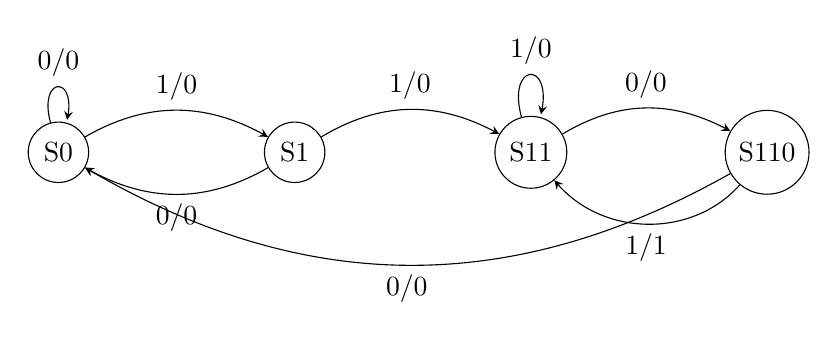
\begin{tikzpicture}[->,>=stealth,node distance=2.8cm,auto]
\node[draw,circle] (S0) at (0,0) {S0};
\node[draw,circle] (S1) at (3,0) {S1};
\node[draw,circle] (S11) at (6,0) {S11};
\node[draw,circle] (S110) at (9,0) {S110};
\draw (S0) edge[loop above] node{0/0} (S0);
\draw (S0) edge[bend left] node{1/0} (S1);
\draw (S1) edge[bend left] node{0/0} (S0);
\draw (S1) edge[bend left] node{1/0} (S11);
\draw (S11) edge[loop above] node{1/0} (S11);
\draw (S11) edge[bend left] node{0/0} (S110);
\draw (S110) edge[bend left=30] node{0/0} (S0);
\draw (S110) edge[bend left=50] node{1/1} (S11);
\end{tikzpicture}
\end{center}

\textbf{【转移表】}
\begin{center}
\begin{tabular}{|c|c|c||c|c|}\hline
当前 & din & 次态 & 输出 \\ \hline
S0 & 0 & S0 & 0 \\ \hline S0 & 1 & S1 & 0 \\ \hline
S1 & 0 & S0 & 0 \\ \hline S1 & 1 & S11 & 0 \\ \hline
S11 & 0 & S110 & 0 \\ \hline S11 & 1 & S11 & 0 \\ \hline
S110 & 0 & S0 & 0 \\ \hline S110 & 1 & S11(重叠) & \textbf{1} \\ \hline
\end{tabular}
\end{center}

\textbf{【VHDL关键转移】}
\begin{lstlisting}
 when S110 =>
  if din = '1' then next_state <= S11;  -- 重叠：最后1→S11
  else next_state <= S0; end if;
\end{lstlisting}

\textbf{【关键分析】}S11+1→S11（"111"中后两个1可作为新的"11"前缀）。
S110+1→检测到→S11（重叠！"1101"最后的"1"→1→"11"中）。

\end{solution}


% ============================================================
\section{题4：检测0101（重叠）}

\textbf{题目}：设计重叠检测0101的状态机。

\begin{solution}[完整解答]

\textbf{【状态】}S0→S01(0)→S010(01)→S0101(检测)→重叠时去S01

\textbf{【转移表】}
\begin{center}
\begin{tabular}{|c|c|c||c|c|}\hline
当前 & din & 次态 & 输出 \\ \hline
S0 & 0 & S01 & 0 \\ \hline S0 & 1 & S0 & 0 \\ \hline
S01 & 0 & S01 & 0 \\ \hline S01 & 1 & S010 & 0 \\ \hline
S010 & 0 & S0101 & 0 \\ \hline S010 & 1 & S0 & 0 \\ \hline
S0101 & 0 & S01 & 0 \\ \hline S0101 & 1 & S010(重叠) & \textbf{1} \\ \hline
\end{tabular}
\end{center}

\textbf{【重叠行为】}S0101+1→检测到。最后的"1"→新序列的第二步（需要前面有0，所以去S01(0已在前一步提供了)）。

不对——仔细分析：
S0101+0→S01（"0"可以是新序列的第一个0）
S0101+1→S010（"1"匹配了序列的第二步"01"中的"1"）

\end{solution}


% ============================================================
\section{题5：检测1111（连续4个1）}

\textbf{题目}：设计重叠检测1111（连续4个1）的状态机。

\begin{solution}[完整解答]

\textbf{【状态】}S0→S1(1个1)→S11(2个1)→S111(3个1)。S111+1→检测到。

\textbf{【关键】}重叠：任何时候输入0→回S0。但S111+1→去S111（"1111"中后3个1可作为新"111"前缀）。

\textbf{【VHDL】}
\begin{lstlisting}
type state_type is (S0, S1, S11, S111);
...
 when S0 =>
  if din = '1' then next_state <= S1; else next_state <= S0; end if;
 when S1 =>
  if din = '1' then next_state <= S11; else next_state <= S0; end if;
 when S11 =>
  if din = '1' then next_state <= S111; else next_state <= S0; end if;
 when S111 =>
  if din = '1' then
    next_state <= S111;  -- 重叠！后3个1仍是有效前缀
  else
    next_state <= S0;
  end if;
\end{lstlisting}

\textbf{【输出】}detected = '1' when state=S111 and din='1'。

\end{solution}


% ============================================================
\section{题6：检测1001（重叠）}

\textbf{题目}：设计重叠检测1001的状态机。

\begin{solution}[完整解答]

\textbf{【状态】}S0→S1(1)→S10(10)→S100(100)。S100+1→检测到→重叠去S1（最后的1是新序列的第一个1）。

\textbf{【关键转移】}
\begin{itemize}
  \item S100+0→S0（"1000"不匹配任何有效前缀）
  \item S100+1→检测到！→S1（重叠：最后的1→新序列第一步）
\end{itemize}

\end{solution}


% ============================================================
\section{题7：检测010（3位序列）}

\textbf{题目}：设计重叠检测010的状态机（3位序列）。

\begin{solution}[完整解答]

\textbf{【状态】}S0→S01(0)→S010(检测)。重叠行为：S010+0→S01（最后的0→新序列第1位）。

\textbf{【转移图】}
\begin{center}
\begin{tikzpicture}[->,>=stealth,node distance=2.5cm]
\node[draw,circle] (S0) at (0,0) {S0};
\node[draw,circle] (S01) at (3,0) {S01};
\node[draw,circle] (S010) at (6,0) {S010};
\draw (S0) edge[loop above] node{1/0} (S0);
\draw (S0) edge[bend left] node{0/0} (S01);
\draw (S01) edge[bend left] node{0/0} (S01);
\draw (S01) edge[bend left] node{1/0} (S010);
\draw (S010) edge[bend left=30] node{1/0} (S0);
\draw (S010) edge[bend left=50] node{0/1} (S01);
\end{tikzpicture}
\end{center}

\textbf{【VHDL】}
\begin{lstlisting}
type state_type is (S0, S01, S010);
signal state : state_type;
begin
  process(clk, rst_n)
  begin
    if rst_n = '0' then state <= S0;
    elsif rising_edge(clk) then
      case state is
        when S0 =>
          if din = '0' then state <= S01; end if;
        when S01 =>
          if din = '1' then state <= S010; end if;
        when S010 =>
          if din = '0' then state <= S01;   -- 重叠!
          else state <= S0; end if;
      end case;
    end if;
  end process;
  detected <= '1' when (state = S010 and din = '0') else '0';
end fsm;
\end{lstlisting}

\end{solution}


% ============================================================
\section{题8：检测101（3位序列）}

\textbf{题目}：设计重叠检测101的状态机。

\begin{solution}[完整解答]

\textbf{【状态】}S0→S1(1)→S10(10)。S10+1→检测到→去S1（最后的1→新序列的第一个1，重叠）。

\textbf{【注意对比】}检测101非重叠：S10+1→检测到→去S0。

\end{solution}


% ============================================================
\section{题9：同时检测1011和1101（合并状态机）}

\textbf{题目}：设计能同时检测1011和1101的状态机。任一检测到，对应输出=1。

\begin{solution}[完整解答]

\textbf{【状态共享】}两个序列共享前缀"1"：
\begin{itemize}
  \item S0→S1(1)→分支：S10(10: 1011的前缀) 或 S11(11: 1101的前缀)
  \item S10→S101(101)→(1→检测到1011)
  \item S11→S110(110)→(1→检测到1101)
\end{itemize}

\textbf{【状态图】}
\begin{center}
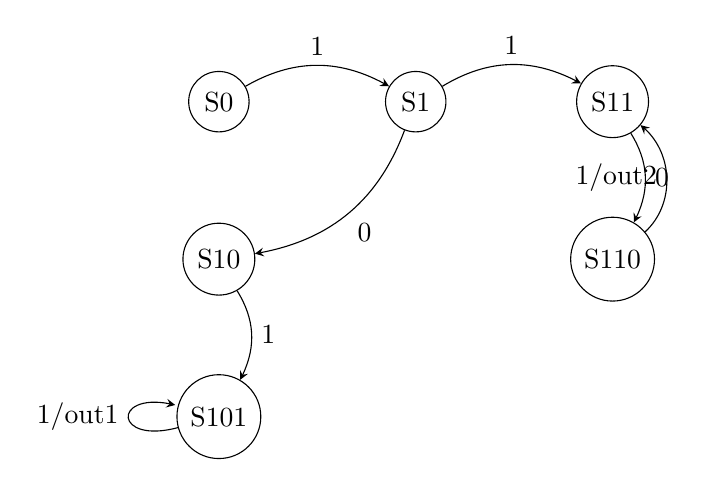
\begin{tikzpicture}[->,>=stealth,node distance=2.3cm,auto]
\node[draw,circle] (S0) at (0,0) {S0};
\node[draw,circle] (S1) at (2.5,0) {S1};
\node[draw,circle] (S10) at (0,-2) {S10};
\node[draw,circle] (S11) at (5,0) {S11};
\node[draw,circle] (S101) at (0,-4) {S101};
\node[draw,circle] (S110) at (5,-2) {S110};
\draw (S0) edge[bend left] node{1} (S1);
\draw (S1) edge[bend left] node{0} (S10);
\draw (S1) edge[bend left] node{1} (S11);
\draw (S10) edge[bend left] node{1} (S101);
\draw (S101) edge[loop left] node{1/out1} (S101);
\draw (S11) edge[bend left] node{0} (S110);
\draw (S110) edge[bend right=50] node{1/out2} (S11);
\end{tikzpicture}
\end{center}

\textbf{【VHDL关键转移】}
\begin{lstlisting}
 when S0 =>
  if din = '1' then state <= S1; end if;
 when S1 =>
  if din = '0' then state <= S10;
  elsif din = '1' then state <= S11; end if;
 when S10 =>
  if din = '1' then state <= S101; else state <= S0; end if;
 when S11 =>
  if din = '0' then state <= S110;
  elsif din = '1' then state <= S11; end if;
 when S101 =>
  if din = '1' then state <= S1;   -- 检测到1011!
  elsif din = '0' then state <= S10; end if;
 when S110 =>
  if din = '1' then state <= S11;  -- 检测到1101!
  elsif din = '0' then state <= S0; end if;
\end{lstlisting}

\end{solution}


% ============================================================
\section{题10：检测序列长度可配置（移位寄存器方案）}

\textbf{题目}：用移位寄存器+比较器实现可配置的序列检测器。目标序列TARGET可动态设置。

\begin{solution}[完整解答]

\textbf{【VHDL】}
\begin{lstlisting}
entity config_detector is
  port (clk, rst_n, din : in std_logic;
        TARGET : in std_logic_vector(3 downto 0);
        detected : out std_logic);
end config_detector;

architecture rtl of config_detector is
  signal reg : std_logic_vector(3 downto 0);
begin
  process(clk, rst_n)
  begin
    if rst_n = '0' then reg <= (others => '0');
    elsif rising_edge(clk) then
      reg <= din & reg(3 downto 1);
    end if;
  end process;
  detected <= '1' when reg = TARGET else '0';
end rtl;
\end{lstlisting}

\textbf{【优点】}无需修改状态机，改变TARGET即可检测任何4位序列。

\textbf{【局限】}自动重叠检测（移位寄存器天然支持重叠）。

\end{solution}


% ============================================================
\section{题11：统计检测次数}

\textbf{题目}：扩展1011检测器，增加计数器统计检测到的总次数（0-255）。

\begin{solution}[完整解答]

\textbf{【VHDL——在检测信号上加计数器】}
\begin{lstlisting}
signal detect_count : integer range 0 to 255;
signal detected : std_logic;

-- 原有状态机代码...
detected <= '1' when (state = S101 and din = '1') else '0';

-- 检测计数器
process(clk, rst_n)
begin
  if rst_n = '0' then detect_count <= 0;
  elsif rising_edge(clk) then
    if detected = '1' then
      detect_count <= detect_count + 1;
    end if;
  end if;
end process;
\end{lstlisting}

\end{solution}


% ============================================================
\section{题12：带超时检测的序列检测器}

\textbf{题目}：若超过16拍未检测到序列，输出timeout。

\begin{solution}[完整解答]

\textbf{【VHDL】}
\begin{lstlisting}
signal timeout_cnt : integer range 0 to 15;
...
process(clk, rst_n)
begin
  if rst_n = '0' then timeout_cnt <= 0;
  elsif rising_edge(clk) then
    if detected = '1' then
      timeout_cnt <= 0;  -- 检测到→清超时计数
    elsif state = S1 then  -- 匹配进行中→保持计数
      timeout_cnt <= timeout_cnt;
    else
      if timeout_cnt = 15 then
        timeout_cnt <= 15;  -- 保持超时
      else
        timeout_cnt <= timeout_cnt + 1;
      end if;
    end if;
  end if;
end process;
timeout <= '1' when timeout_cnt = 15 else '0';
\end{lstlisting}

\end{solution}


% ============================================================
\section{题13：Moore型 vs Mealy型对比}

\textbf{题目}：分别写出检测1011的Moore型和Mealy型状态机，比较异同。

\begin{solution}[完整解答]

\begin{center}
\begin{tabular}{|l|c|c|}\hline
 & Moore型 & Mealy型 \\ \hline
输出决定因素 & 仅当前状态 & 状态+输入 \\ \hline
状态数 & 多(需"检测到"状态) & 少(检测在转移上) \\ \hline
检测延迟 & 晚1拍 & 同1拍 \\ \hline
输出稳定性 & 全周期稳定 & 输入变化时可能抖 \\ \hline
考试推荐 & 更安全 & 更快 \\ \hline
\end{tabular}
\end{center}

\textbf{【Mealy型VHDL（更简洁）】}
\begin{lstlisting}
-- Mealy: 输出在转移中表达
 when S101 =>
  if din = '1' then
    next_state <= S1; detected <= '1';  -- Mealy输出
  else
    next_state <= S10; detected <= '0';
  end if;
\end{lstlisting}

\textbf{【推荐】}考试如无特别说明，用Moore型。更稳定，状态图更清晰。

\end{solution}


% ============================================================
\section{题14：4位并行序列检测}

\textbf{题目}：输入是4位并行数据，检测特定4位模式（如"1011"）。每拍判断一次。

\begin{solution}[完整解答]

\textbf{【分析】}纯组合逻辑！不需要状态机。$detected = '1'$ when $data\_in = "1011"$。

\textbf{【VHDL】}
\begin{lstlisting}
entity parallel_detect is
  port (data_in : in std_logic_vector(3 downto 0);
        detected : out std_logic);
end parallel_detect;

architecture rtl of parallel_detect is
begin
  detected <= '1' when data_in = "1011" else '0';
end rtl;
\end{lstlisting}

\textbf{【与串行检测的本质区别】}并行检测不需要记忆历史——当前4位数据同时可见。串行检测需要状态机或移位寄存器来"记住"历史。

\end{solution}


% ============================================================
\section{题15：检测包含"无关位"的序列}

\textbf{题目}：检测1xx1（第1位和第4位为1，中间两位任意）。

\begin{solution}[完整解答]

\textbf{【移位寄存器方案】}
\begin{lstlisting}
detected <= '1' when reg(3) = '1' and reg(0) = '1' else '0';
-- 只检查第1位和第4位
\end{lstlisting}

\textbf{【状态机方案】}
状态S1→S1x→S1xx→S1xx1(检测)。中间两位任意值都接受。

\end{solution}


% ============================================================
\section{题16：给定状态图写VHDL}

\textbf{题目}：给定下面状态图，写出完整VHDL状态机。

\begin{center}
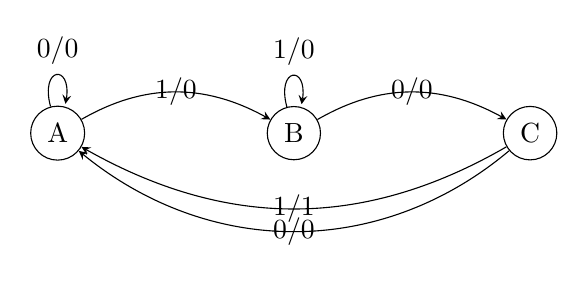
\begin{tikzpicture}[->,>=stealth,node distance=2.5cm]
\node[draw,circle] (A) at (0,0) {A};
\node[draw,circle] (B) at (3,0) {B};
\node[draw,circle] (C) at (6,0) {C};
\draw (A) edge[bend left] node{1/0} (B);
\draw (A) edge[loop above] node{0/0} (A);
\draw (B) edge[bend left] node{0/0} (C);
\draw (B) edge[loop above] node{1/0} (B);
\draw (C) edge[bend left=40] node{0/0} (A);
\draw (C) edge[bend left] node{1/1} (A);
\end{tikzpicture}
\end{center}

\begin{solution}[完整解答]

\textbf{【从图到代码的映射】}
箭头标注 X/Y = 输入/输出。

\textbf{【VHDL】}
\begin{lstlisting}
type state_type is (A_state, B_state, C_state);
signal state : state_type;
begin
  process(clk, rst_n)
  begin
    if rst_n = '0' then state <= A_state;
    elsif rising_edge(clk) then
      case state is
        when A_state =>
          if din = '1' then state <= B_state; end if;
          -- din='0': 保持A_state (loop above)
        when B_state =>
          if din = '0' then state <= C_state; end if;
          -- din='1': 保持B_state (loop above)
        when C_state =>
          state <= A_state;  -- 无论0还是1都回A
      end case;
    end if;
  end process;
  detected <= '1' when (state = C_state and din = '1') else '0';
end fsm;
\end{lstlisting}

\end{solution}


% ============================================================
\section{题17：给定输入序列和状态机，求输出序列}

\textbf{题目}：1011检测器（重叠），输入=1011011。求输出序列。

\begin{solution}[完整解答]

\textbf{【逐拍追踪】}
\begin{center}
\begin{tabular}{|c|c|c|c|c|c|c|c|}\hline
拍 & 1 & 2 & 3 & 4 & 5 & 6 & 7 \\ \hline
din & 1 & 0 & 1 & 1 & 0 & 1 & 1 \\ \hline
状态(当前) & S0 & S1 & S10 & S101 & S1 & S10 & S101 \\ \hline
状态(次态) & S1 & S10 & S101 & S1 & S10 & S101 & S1 \\ \hline
输出 & 0 & 0 & 0 & \textbf{1} & 0 & 0 & \textbf{1} \\ \hline
\end{tabular}
\end{center}

输出序列：\textbf{0 0 0 1 0 0 1}

\begin{itemize}
  \item 第4拍：S101+1→检测1011！→重叠去S1
  \item 第7拍：S101+1→再次检测1011！→重叠去S1
\end{itemize}

\end{solution}


% ============================================================
\section{题18：状态编码优化}

\textbf{题目}：1011检测器4个状态。分别用Binary(2位)和One-hot(4位)编码。哪个体积更小？哪个速度更快？

\begin{solution}[完整解答]

\textbf{【Binary编码（2位DFF）】}
\begin{center}
\begin{tabular}{|c|c|}\hline
状态 & 编码 \\ \hline
S0 & 00 \\ \hline S1 & 01 \\ \hline
S10 & 10 \\ \hline S101 & 11 \\ \hline
\end{tabular}
\end{center}
优点：2个DFF（面积小）。缺点：需要译码电路（速度慢）。

\textbf{【One-hot编码（4位DFF）】}
\begin{center}
\begin{tabular}{|c|c|}\hline
状态 & 编码 \\ \hline
S0 & 0001 \\ \hline S1 & 0010 \\ \hline
S10 & 0100 \\ \hline S101 & 1000 \\ \hline
\end{tabular}
\end{center}
优点：无需译码（速度快）。缺点：4个DFF（面积大）。

\textbf{【考试答案】}面积最小→Binary。速度最快→One-hot。

\textbf{【FPGA实际】}综合工具默认自动选择最优编码，你不需要手动指定。

\end{solution}


% ============================================================
\section{题19：序列检测器模板化}

\textbf{题目}：编写检测任意4位序列的通用VHDL模板（参数化：TARGET可配置）。

\begin{solution}[完整解答]

\textbf{【状态机通用模板】}
\begin{lstlisting}
entity seq_detector_generic is
  generic (TARGET : std_logic_vector(3 downto 0));
  port (clk, rst_n, din : in std_logic; detected : out std_logic);
end seq_detector_generic;

architecture fsm of seq_detector_generic is
  type state_type is (S0, S1, S2, S3);
  signal state : state_type;
begin
  process(clk, rst_n)
  begin
    if rst_n = '0' then state <= S0;
    elsif rising_edge(clk) then
      case state is
        when S0 =>
          if din = TARGET(3) then state <= S1; end if;
        when S1 =>
          if din = TARGET(2) then state <= S2;
          elsif din = TARGET(3) then state <= S1;
          else state <= S0; end if;
        when S2 =>
          if din = TARGET(1) then state <= S3;
          elsif din = TARGET(3) then state <= S1;
          else state <= S0; end if;
        when S3 =>
          if din = TARGET(0) then state <= S1;  -- 检测+重叠
          elsif din = TARGET(3) then state <= S1;
          else state <= S0; end if;
      end case;
    end if;
  end process;
  detected <= '1' when (state = S3 and din = TARGET(0)) else '0';
end fsm;
\end{lstlisting}

\textbf{【使用】}generic map(TARGET=>"1011")即可检测1011。

\end{solution}


% ============================================================
\section{题20：序列检测器秒杀总结}

\begin{quickkill}[序列检测器——考试必考，20题统一解法]

\textbf{第一步：状态 = 已匹配的前缀}
\begin{itemize}
  \item 每个状态代表"已匹配了目标序列的前几位"
  \item N位序列 → 最多N个状态（不含初始S0）
\end{itemize}

\textbf{第二步：画状态转移图}
对每个状态，考虑输入0和输入1分别：
\begin{itemize}
  \item 匹配推进：去下一个状态
  \item 匹配失败：找最长的"已匹配后缀"作为新状态
  \item 检测到：输出=1
\end{itemize}

\textbf{第三步：确定重叠/非重叠}
\begin{itemize}
  \item \textbf{重叠：}检测到后→检查最后的输入能否构成新前缀
  \item \textbf{非重叠：}检测到后→回S0
\end{itemize}

\textbf{第四步：写VHDL（三段式Moore型）}
\begin{enumerate}
  \item 状态寄存器：process(clk,rst) + rising\_edge
  \item 次态逻辑：process(state,din) + case
  \item 输出逻辑：并行信号赋值
\end{enumerate}

\textbf{常考序列状态数速查：}
\begin{itemize}
  \item 1011 → 4状态(S0,S1,S10,S101)
  \item 1101 → 4状态(S0,S1,S11,S110)
  \item 1111 → 4状态(S0,S1,S11,S111)
  \item 0101 → 4状态(S0,S01,S010,S0101)
  \item 101 → 3状态(S0,S1,S10)
  \item 010 → 3状态(S0,S01,S010)
\end{itemize}

\textbf{VHDL状态机模板（一行不改，只换状态名和转移逻辑）}
\begin{lstlisting}
type state_type is (...);
signal state : state_type;
process(clk, rst_n)
begin
  if rst_n='0' then state <= S0;
  elsif rising_edge(clk) then
    case state is
      when S0 => if din='1' then state <= S1; end if;
      ...
    end case;
  end if;
end process;
detected <= '1' when (...) else '0';
\end{lstlisting}

\textbf{速胜法宝：移位寄存器替代方案}
序列长度≤8位时，用移位寄存器+比较器实现序列检测比状态机简单得多！

\begin{lstlisting}
reg <= din & reg(N-1 downto 1);
detected <= '1' when reg = TARGET else '0';  -- 一行搞定！
\end{lstlisting}

\textbf{但注意：考试如果明确要求"用状态机设计"，则必须用状态机！}
\end{quickkill}


\end{document}
